%% Le lingue utilizzate, che verranno passate come opzioni al pacchetto babel. Come sempre, l'ultima indicata sar� quella primaria.
%% Se si utilizzano una o pi� lingue diverse da "italian" o "english", leggere le istruzioni in fondo.
\def\thudbabelopt{english}
%% Valori ammessi per target: bach (tesi triennale), mst (tesi magistrale), phd (tesi di dottorato).
\documentclass[target=bach]{thud}[2014/03/11]
\usepackage{adjustbox}
\usepackage{tabularx, colortbl}
\usepackage{float}
\usepackage{hyperref}
\usepackage{graphicx}
%\usepackage{bera}% optional: just to have a nice mono-spaced font
\usepackage{listings}
\usepackage{xcolor}
%\usepackage{natbib}
\usepackage{algpseudocode}
\usepackage{tocbibind}
\usepackage{mathtools}
\usepackage{algorithmicx}
\usepackage{algorithm}
%\usepackage{cite}
\usepackage{dirtytalk}
\usepackage{amssymb}% http://ctan.org/pkg/amssymb
\usepackage{pifont}% http://ctan.org/pkg/pifont
\newcommand{\cmark}{\ding{51}}%
\newcommand{\xmark}{\ding{55}}
\newcommand{\greenc}{{\color{green}\cmark}}
\newcommand{\orangec}{{\color{orange}\cmark}}
\newcommand{\redx}{{\color{red}\xmark}}

\definecolor{lightgray}{rgb}{0.95, 0.95, 0.95}
\definecolor{darkgray}{rgb}{0.4, 0.4, 0.4}
%\definecolor{purple}{rgb}{0.65, 0.12, 0.82}
\definecolor{editorGray}{rgb}{0.95, 0.95, 0.95}
\definecolor{editorOcher}{rgb}{1, 0.5, 0} % #FF7F00 -> rgb(239, 169, 0)
\definecolor{editorGreen}{rgb}{0, 0.5, 0} % #007C00 -> rgb(0, 124, 0)
\definecolor{orange}{rgb}{1,0.45,0.13}		
\definecolor{olive}{rgb}{0.17,0.59,0.20}
\definecolor{brown}{rgb}{0.69,0.31,0.31}
\definecolor{purple}{rgb}{0.38,0.18,0.81}
\definecolor{lightblue}{rgb}{0.1,0.57,0.7}
\definecolor{lightred}{rgb}{1,0.4,0.5}

\lstdefinelanguage{JavaScript}{
  morekeywords={typeof, new, true, false, catch, function, return, null, catch, switch, var, if, in, while, do, else, case, break},
  morecomment=[s]{/*}{*/},
  morecomment=[l]//,
  frame=lines,
  morestring=[b]",
  morestring=[b]'
}

\colorlet{punct}{red!60!black}
\definecolor{background}{HTML}{EEEEEE}
\definecolor{delim}{RGB}{20,105,176}
\colorlet{numb}{magenta!60!black}
\definecolor{color:keyword}{rgb}{0.53,0.05,0.05}
\definecolor{color:comment}{rgb}{0.25,0.37,0.75}
\definecolor{color:string}{rgb}{0.87,0.0,0.0}

\lstdefinelanguage{Jolie}{
 morekeywords={csets,type,raw,any,undefined,void,default,if,for,while,spawn,foreach,else,define,main,include,constants,inputPort,outputPort,interface,execution,cset,nullProcess,RequestResponse,OneWay,throw,throws,install,scope,embedded,init,synchronized,global,is_defined,is_int,is_bool,is_long,is_string,bool,long,int,string,double,undef,with,Location,Protocol,Interfaces,Aggregates,Redirects,linkIn,linkOut},
 sensitive=true,
 morecomment=[l]{//},
 morecomment=[s]{/*}{*/},
 morestring=[b]",
 otherkeywords={;,|,@}
}

\lstset{
 language=Jolie,
 mathescape=true,
 resetmargins=true,
 numberstyle=\footnotesize,
 numbers=left,
 numbersep=5pt,
 numberblanklines=true,
 basicstyle=\ttfamily\small,
 tabsize=2,
 frame=lines,
 commentstyle=\ttfamily\color{color:comment},
 stringstyle=\color{color:string},
 captionpos=b,
 keywordstyle=\bfseries\color{color:keyword},
 showstringspaces=false,
 belowcaptionskip=10mm,
 breaklines=false,
 columns=fullflexible,
 linewidth= 0.8\linewidth,
 mathescape=false,
 literate=*{\$}{{{\textcolor{black}\$}}}{1}
}


\colorlet{punct}{red!60!black}
\definecolor{keyword}{RGB}{48,0,211}
\colorlet{numb}{magenta!60!black}

\newcommand{\kwd}[1]{{\color{keyword}\textbf{#1}}}
\newcommand{\hid}[1]{{\color{gray}#1}}

\lstdefinelanguage{json}{
    basicstyle=\ttfamily\small,
    commentstyle=\color{color:comment}, % style of comment
    stringstyle=\color{color:string}, % style of strings
    numbers=left,
    numberstyle=\scriptsize,
    stepnumber=1,
    numbersep=8pt,
    showstringspaces=false,
    frame=lines,
    string=[s]{"}{"},
    comment=[l]{:\ "},
    morecomment=[l]{:"},
    mathescape=false,
    literate=
        *{0}{{{\color{numb}0}}}{1}
         {1}{{{\color{numb}1}}}{1}
         {2}{{{\color{numb}2}}}{1}
         {3}{{{\color{numb}3}}}{1}
         {4}{{{\color{numb}4}}}{1}
         {5}{{{\color{numb}5}}}{1}
         {6}{{{\color{numb}6}}}{1}
         {7}{{{\color{numb}7}}}{1}
         {8}{{{\color{numb}8}}}{1}
         {9}{{{\color{numb}9}}}{1}
         {\$}{{{\color{numb}\$}}}{1}         
}
%\lstdefinelanguage{json}{
%    basicstyle=\normalfont\ttfamily,
%    numbers=left,
%    numberstyle=\scriptsize,
%    stepnumber=1,
%    numbersep=8pt,
%    showstringspaces=false,
%    breaklines=true,
%    frame=lines,
%    backgroundcolor=\color{background},
%    literate=
%     *{0}{{{\color{numb}0}}}{1}
%      {1}{{{\color{numb}1}}}{1}
%      {2}{{{\color{numb}2}}}{1}
%      {3}{{{\color{numb}3}}}{1}
%      {4}{{{\color{numb}4}}}{1}
%      {5}{{{\color{numb}5}}}{1}
%      {6}{{{\color{numb}6}}}{1}
%      {7}{{{\color{numb}7}}}{1}
%      {8}{{{\color{numb}8}}}{1}
%      {9}{{{\color{numb}9}}}{1}
%      {:}{{{\color{punct}{:}}}}{1}
%      {,}{{{\color{punct}{,}}}}{1}
%      {\{}{{{\color{delim}{\{}}}}{1}
%      {\}}{{{\color{delim}{\}}}}}{1}
%      {[}{{{\color{delim}{[}}}}{1}
%      {]}{{{\color{delim}{]}}}}{1},
%}


%% --- Informazioni sulla tesi ---
%% Per tutti i tipi di tesi
\title{Design and implementation of a Language Server for the Jolie programming language}
\author{Eros Fabrici}
\course{Tecnologie Web e Multimediali}
\supervisor{Prof.\ Marino Miculan}
%% Altri campi disponibili: \reviewer, \tutor, \chair, \date (anno accademico, calcolato in automatico).
%% Con \supervisor, \cosupervisor, \reviewer e \tutor si possono indicare pi� nomi separati da \and.
%% Per le sole tesi di dottorato
%%\phdnumber{313}
%%\cycle{XXVIII}
%%\contacts{Via della Sintassi Astratta, 0/1\\65536 Gigatera --- Italia\\+39 0123 456789\\\texttt{http://www.example.com}\\\texttt{inbox@example.com}}
%%\rights{Tutti i diritti riservati a me stesso e basta.}
%% Campi obbligatori: \title, \author e \course.

%% --- Pacchetti consigliati ---
%% hyperref: Regola le impostazioni della creazione del PDF... pi� tante altre cose.
%% tocbibind: Inserisce nell'indice anche la lista delle figure, la bibliografia, ecc.

%% --- Stili di pagina disponibili (comando \pagestyle) ---
%% sfbig (predefinito): Apertura delle parti e dei capitoli col numero grande; titoli delle parti e dei capitoli e intestazioni di pagina in sans serif.
%% big: Come "sfbig", solo serif.
%% plain: Apertura delle parti e dei capitoli tradizionali di LaTeX; intestazioni di pagina come "big".

\begin{document}

%% Il frontespizio prima di tutto!
\maketitle

%% Dedica (opzionale)
\begin{dedication}Alla mia famiglia,\par per avermi supportato in ogni mia decisione.\end{dedication}

%% Ringraziamenti (opzionali)
\acknowledgements
First of all, I would like to thank my thesis supervisor, Professor Marino Miculan both for his suggestions for this thesis, and for his help in organizing my university exchanges abroad.

I would like also to thank Professor Fabrizio Montesi and PhD Saverio Giallorenzo, from the University of Southern Denmark, for supervising me during my internship in Odense.

Finally, I would like to thank my family, my friends and my girlfriend, who supported me over the last few years. 
%Innanzitutto, vorrei ringraziare il Professor Marino Miculan, relatore di questa tesi, sia per i suggerimenti fornitomi per la stesura, sia per avermi aiutato ed indirizzato durante i miei due scambi all'estero.

%Vorrei anche ringraziare il Professor Fabrizio Montesi e il Dott. Saverio Giallorenzo della University of Southern Denmark per avermi seguito ed aiutato durante il mio Erasmus+ Traineeship.

%Infine, vorrei ringraziare la mia famiglia, i miei amici e la mia morosa, per avermi supportato in questi anni e ai quali dedico questo lavoro.
%Infine, vorrei ringraziare le persone a me pi� care: la mia famiglia, i miei amici e la mia morosa, per avermi supportato in questi anni e ai quali dedico questo lavoro.

%% Indice
\tableofcontents

%% Lista delle tabelle (se presenti)
\listoftables

%% Lista delle figure (se presenti)
\listoffigures

%% Corpo principale del documento
\mainmatter

%% Parte
%% La suddivisione in parti � opzionale; talvolta sono sufficienti i capitoli.

%% Capitolo
\chapter{Introduction}
%%Problem: implementing advance IDE functionalities for the Jolie language to be added in Microsoft Vs-code and similar
Service-Oriented Computing (SOC) is the computing paradigm that utilizes services as fundamental elements for developing applications/solutions. A \emph{service} is an independent software entity that can be accessed remotely by other services through message passing. To build the service model, SOC relies on the Service Oriented Architecture (SOA) \cite{Papazoglou03service-orientedcomputing:} which is a software design technique, used to represent a distributed system based on services. In the last decade a SOA variant emerged, called \emph{Microservices}, which is a software development technique where an application is a collection of loosely coupled, fine-grained services that communicate with lightweight protocols over well-defined APIs. In other words, this architecture model describes a particular way of designing software applications as suites of independently deployable services \cite{msFowler}. Microservices are getting more very popular over the years, with growing international communities, such as the Microservices Community \cite{msCommunity}, and multinational corporations providing platforms for developing those kind of applications, for instance Amazon AWS and Google Cloud provide platforms where users can deploy their microservice architectures.

SOC abstracts from the implementation details of services by imposing a standard communication mechanism between the entities in an SOA \cite{Jol}. From the perspective of these architectures, it is possible to identify a separation between \textit{behavioral} and \textit{architectural} composition of services. The first denotes a series of interactions to be performed in order to reach a goal, while the second deals with the topological structure of a SOA/microservices architecture, managing its execution and integration. The lack of a homogeneous solution between the \textit{behavioral} and the \textit{architectural} composition of services require ad-hoc interventions in order to integrate them, which will make the entire architecture less modular and difficult to maintain. \emph{Jolie} \cite{Montesi_coorg2006, Jolie} was created with the intention to fill this gap. This language permits to define services, their behavioral composition, supporting different communication technologies and their organization inside a microservices architecture.

Since the usage of Jolie is growing, both in academia and in industry \cite{JAcad}, it is necessary to provide tools which aim is to ease rapid and correct design and development. Regarding the latter, it is important that the editor used supports functionalities like auto completion, hover information, linting, etc.. Nowadays there is no such an editor for Jolie.

The aim of this thesis is to design and implement a software tool which provides these features to be integrated in commonly used editors, like Visual Studio Code and Atom. Implementing such a tool, can take a significant effort. Traditionally this work had to be repeated for each development tool, as each of them provides different APIs for implementing the same feature \cite{LSPIntro}. Therefore, the solution proposed is to use the \emph{Language Server Protocol} (LSP) by Microsoft, which aim is to standardize the communication between an IDE and a server, referred as \emph{Language Server} (LS), that provides language-specific features. This solves the problem presented above: with a LS that supports the LSP, the first can be re-used in multiple development tools that support the protocol.

The thesis is the result of a 4 months internship at the University of Southern Denmark, with the Concurrency and Logic research team \cite{C&L} under the supervision of Professor Fabrizio Montesi \cite{MontesiWP}, which is the Jolie project leader and maintainer.

This thesis is structured as it follows. In Chapter 2 we present the Jolie language, by describing its syntax and showing some practical examples, and the Language Server Protocol, where we describe the protocol and its features. In Chapter 3 we analyze the problem and elicitate the requirements, both functional and non-functional ones. Chapter 4 presents two possible architectures for the LS, followed by a brief description of their components. In Chapter 5 we provide an overview of the implementation, justifying choices made and the problems challenges encountered. Chapter 6 is dedicated to the validation phase, where we show some example of interaction and list which requirements were met. Finally, Chapter 7 outlines the conclusions, where we present a review of the project, what still needs to be completed and some directions for future work.


\chapter{Jolie and the Language Server Protocol}
\label{sec:JolieLSP}
\section{Jolie: Java Orchestration Language Interpreter Engine}
A Jolie program defines a service, which is composed by two parts: the \textit{behavior} and the \textit{deployment}. The first defines the functionalities of the service, including primitives like communication and computation constructs. These does not define \textit{how} the communication is supported, they abstractly refer to \textit{communication ports} which are assumed to be correctly defined in the deployment part. For example, a behavioral primitive may express the action \say{ask the bank to show the actual balance}, without knowing how to reach the \say{bank} service and which communication protocol it uses. These last two are handled by the deployment, which permits to define the \textit{location} and the \textit{protocol} of the bank service. Furthermore, the deployment permits the usage of architectural primitives for defining the architecture of a SOA. The syntax of a Jolie program is defined as shown in Figure \ref{Jsynt1}, where D is the Deployment and B is the Behavior. The \textcolor{color:keyword}{main} procedure is the execution entry point.
\begin{figure}[t]
	\[Program \quad \Coloneqq \quad	D \quad \textcolor{color:keyword}{main}\,\{\, B\, \}\]
	\caption{Jolie Syntax}
	\label{Jsynt1}
\end{figure}
\subsection{Behavior}
Jolie syntax is a combination of the message passing and the imperative programming styles. 
Figure \ref{Bsyntax} lists a selection of the Jolie behavioral syntax:
\begin{figure}[t]
\begin{align*}
	B \quad \Coloneqq&\, \eta \quad (input)\\
	|& \, \bar{\eta} \quad (output)\\
	|& \, \textcolor{color:keyword}{if}(e) \> B_1 \> \big[\textcolor{color:keyword}{else} \> B_2\big] \quad (condition)\\
	|& \, \textcolor{color:keyword}{while}(e) \> B \quad (while)\\
	|& \, \textcolor{color:keyword}{for}(init,\,cond,\,incr)\> B \quad (forLoop)\\
	|& \, \textcolor{color:keyword}{for}(x \, \textcolor{color:keyword}{in} \, y)\> B \quad (arrayIteration)\\
	|& \, B_1 \, ; \, B_2 \quad (sequential)\\
	|& \, B_1 \, | \, B_2 \quad (parallel)\\
	|& \, \{\, B \,\} \quad (block)\\
	|& \, x\,=\,e \quad (assign)\\
	|& \, a\,->\,e \quad (alias)\\
	|& \, x \, << \, y \quad (deepCopy)\\
	|& \, \big[\,\eta_1\,\big]\>\{\,B_1\,\}\,...\, \big[\,\eta_n\,\big]\>\{\,B_n\,\} \quad (inputChoice)\\
	|& \, \textcolor{color:keyword}{scope}(s) \> \{\,B\,\} \quad (scope)\\
	|& \, \textcolor{color:keyword}{install}(\,h_1\> => \>B_1,...,\,h_n\> => \> B_n) \quad (install)\\
	|& \, \textcolor{color:keyword}{throw}(f[,\,x]) \quad (throw)
\end{align*}
%	|& \, \textcolor{color:keyword}{cH} \quad (cH)\\
where
\begin{align*}
	\eta \quad \Coloneqq&\, opName(x) \quad (OneWay)\\
	|& \, opName(x)(e)\>\{\,B\,\} \quad (RequestResponse)
\end{align*}\\
and
\begin{align*}
	\bar{\eta} \quad \Coloneqq&\, opName\textcolor{color:keyword}{@}OP(e) \quad (notification)\\
	|&\, opName\textcolor{color:keyword}{@}OP(e)(x) \quad (SolcitResponse)
\end{align*}
\caption{Behavior syntax}
\label{Bsyntax}
\end{figure}
\subsubsection{Communications}
Communications are implemented by \textit{(input)}, \textit{(output)} and \textit{(inputChoice)} constructs. Input $\boldsymbol\eta$ can be either a \textit{OneWay} or a \textit{RequestResponse}. The first receives a message for the operation \textit{opName} and saves its content in variable \verb|x|, while the second receives a message for operation \textit{opName} in variable \verb|x|, executes behavior \textit{B} and sends the value of the evaluation of the expression \textit{e} to the invoker. \textit{(notification)} and \textit{(SolcitResponse)} implement the output towards the input. The first sends a message with the evaluation of \textit{e}, the second does the same thing and waits for the response from the invoked service which is stored in the var \verb|x|. \textit{OP} denotes the \textbf{output port name} that references an \textcolor{color:keyword}{outputPort}. The latter is specified in the deployment definition and it contains all the necessary information in order to contact the target service. Lastly, the \textit{(inputChoice)} supports the receiving of a message for any of the inputs. When a message for the input $\eta_i$ is received, all the remaining branches are deactivated and $\eta_i$ is executed. Afterwards, $B_i$ is executed. The interpreter enforces that $\eta_i \neq \eta_j,\,\forall i,j \in [1,n] \, | \, i \neq j$, which means that there cannot be two inputs with the same operation.

\paragraph{Statment compositions.} \textit{(condition)}, \textit{(while)}, \textit{(forLoop)}, \textit{(arrayIteration)} and \textit{(block)}, resembles the ones used in classic imperative styles. Rule \textit{sequential} sequentially compose the two behaviors: when $B_1$ is terminated, $B_2$ can start its execution (remark: the separator \textit{;} is now optional). On the contrary, \textit{(parallel)} permits the parallel execution of the two behaviors.

\paragraph{Assignment and aliasing.} \textit{(assign)} evaluates the expression \textit{e} and assigns its value to the variable \verb|x|. \textit{(alias)} permits to define a variable $a$ that points to $x$ variable path.

\paragraph{Handling data.} Jolie is dynamically-typed meaning that there is no necessity of type declarations and that the type of a variable value is checked at runtime. The language handles the following basic data types:
\begin{itemize}
	\item \verb|bool|: booleans;
	\item \verb|int|: integers;	
	\item \verb|long|: long integers (with \verb|l| or \verb|L| suffix);
	\item \verb|double|: double-precision float;
	\item \verb|string|: strings;
	\item \verb|raw|: byte arrays (supported for data-passing purposes);
	\item \verb|void|: the empty type.
\end{itemize}
Jolie supports basic arithmetic and logic operators like in Java and also pre-/post-increment and pre-/post-decrement operators. Furthermore, it is possible to cast variables to other types with the following casting functions: \verb|bool()|, \verb|int()|, \verb|long()|, \verb|double()| and \verb|string()|. For instance:
\begin{lstlisting}[language=Jolie]
	d = "1.5"
	n = double( d ) // n = 1.5
	n = int( n ) // n = 1
\end{lstlisting}
A variable type can be checked at run-time with the \textcolor{color:keyword}{instanceof} operator, whose syntax is:
\[expression \>\> \textcolor{color:keyword}{instanceof} \>\> (native\_type\,|\,custom\_type)\]
Variables are undefined until they are assigned a value. Until then, their state is set to \textcolor{color:keyword}{undefined} (equivalent to \verb|NULL|, \verb|null| or \verb|nil| in other languages). The predicate \textcolor{color:keyword}{is\_defined} is used for checking is a variable is defined or not. Following the syntax:
\[ \textcolor{color:keyword}{is\_defined} (\, variable\_name \,)\]
An example:
\begin{lstlisting}[language=Jolie]
	x = 2
	if ( is_defined( x ) ) {
		println@Console( "Variable x is defined" )
	}
\end{lstlisting}
Arrays in Jolie are handled dynamically and can be accessed using the \verb|[]| operator. To be more precise, in Jolie \textbf{every} variable is a dynamic array. So for example this assignment
\begin{lstlisting}[language=Jolie]
	x = 7
\end{lstlisting}
is equivalent to the following
\begin{lstlisting}[language=Jolie]
	x[0] = 7
\end{lstlisting}
thus managing complex data is easier. To compute the size of an array Jolie provides the size operator \verb|#|. Together with this operator, the \textit{forLoop} can be used to traverse an array. Alternatively, \textit{(arrayIteration)} has the same purpose. The example below shows the usage of the mentioned constructs.
\begin{lstlisting}[language=Jolie]
	x[0] = 1
	x[1] = 2
	x[2] = 3
	println@Console( #x )() // prints 3
	
	for( i = 0, i < #x, i++) {
		println@Console( x[i] )()	
	}
	//which is equivalent to
	for( el in x ) {
		println@Console( el )()	
	}
\end{lstlisting}
\subsubsection{Data Structures}
Data structures in Jolie are tree-like, similarly to XML or JSON data trees. The operator \verb|.| is used to traverse a data structure. Following an example.
\begin{lstlisting}[language=Jolie]
	doctor.name = "Marco"
	doctor.surname = "Rossi"
	doctor.age = 45
	doctor.specialization[0] = "Cardiology"
	doctor.specialization[1] = "General Surgery"
\end{lstlisting}
The above data tree is characterized by \verb|doctor| as root with \verb|void| type and by three children: \verb|name|, \verb|surname|, \verb|age| and \verb|specialization| which respectively have the types \verb|string|, \verb|string|, \verb|int| and \verb|string|. The \textcolor{color:keyword}{undef} operator is used to erase an entire structure. Syntax:
\[\textcolor{color:keyword}{undef}(\,variable\_name\,) \]
The \textit{(deepCopy)} operator copies the entire structure of a tree $y$ into a tree $x$. Jolie at run-time explores the tree $y$ node-wise and for all initialized sub-nodes in $y$, it assigns the value of each of them to the corresponding sub-node rooted in $x$. This means that if $x$ already had sub-nodes initialized that match to some ones rooted in $y$, $x \, << \, y$ will overwrite them, leaving all the others initialized nodes of $x$ unaffected. This operator can be used also as syntax sugar for creating a data structure. Basing on the previous example of the doctor data structure, in can be re-written as in the following example.
\begin{lstlisting}[language=Jolie]
	doctor << {
		name = "Marco"
		surname = "Rossi"
		birthDate << {
			day = 25
			month = 5
			year = 1971
		}
		specialization[0] = "Cardiology"
		specialization[1] = "General Surgery"
		email = "marco.rossi@gmail.com"
	}
\end{lstlisting}
\subsubsection{Fault handling}
Jolie has constructs to handle faults. The primitives meant for this purpose are: \textcolor{color:keyword}{scope}, \textcolor{color:keyword}{install} and \textcolor{color:keyword}{throw}. For more details see \cite{Jol, JolieDoc}.
\subsection{Deployment}
The deployment is the part of a Jolie program in which all the necessary information for establishing communication channels between services are established. The basic primitives are \textit{input ports} and \textit{output ports} which are based on \textit{data types} and \textit{interfaces}. A deployment $D$ is simply a list of deployment instructions among which we can have input and output ports, type definitions, and interfaces \cite{Jol}:
%{\setstretch{0.4}
\begin{align*}
	D \>\> \Coloneqq& \>\> IP \quad (inputPort)\\
	|& \> OP \quad (outputPort)\\
	|& \> T_{def} \quad (typeDefinition)\\
	|& \> I \quad (interface)\\
	|& \> \textcolor{color:keyword}{execution}\{\, M \,\}\\
	|& \> E
\end{align*}
%}
\subsubsection{Communication ports}
Communication ports are primitives that define \textit{how} communications with other services are handled. There are two kind of ports. $(inputPort)$ that exposes input operations to other services. Alternatively, $(outputPort)$ permits the invocation of other services' operations.\\The syntax for input and output port is the following.
%{\setstretch{0.4}
\begin{align*}
	IP \quad \Coloneqq \> &\textcolor{color:keyword}{inputPort}: \, id \> \{\\
	&\textcolor{color:keyword}{location}: \, URI\\
	&\textcolor{color:keyword}{protocol}: \, p\\
	&\textcolor{color:keyword}{interfaces}: \, I_1,\,I_2,...,\,I_n\\
	& \big[ \textcolor{color:keyword}{aggregates}: OPid_1,...,OPid_n\big]\\
	&\}
\end{align*}
\begin{align*}
	OP \quad \Coloneqq \> &\textcolor{color:keyword}{outputPort}: \, id \> \{\\
	&\textcolor{color:keyword}{location}: \, URI\\
	&\textcolor{color:keyword}{protocol}: \, p\\
	&\textcolor{color:keyword}{interfaces}: \, I_1,\,I_2,...,\,I_n\\
	&\}
\end{align*}
%}
These ports are based on three concepts of $location$, $protocol$ and $interface$. The former two define the concrete binding between the program and other services. In particular the $location$ must specify the communication medium. The mediums supported are: \textit{local} (jolie in-memory communication), \textit{socket}, \textit{btl2cap} (Bluetooth L2CAP), \textit{rmi} (Java RMI) and \textit{localsocket} (Unix local sockets). The $protocol$ indicates the data format. Jolie supports the following protocols: \textit{HTTP}, \textit{HTTPS}, \textit{JSON-RPC}, \textit{XML-RPC}, \textit{SOAP}, \textit{SODEP} (created and developed for Jolie), \textit{SODEPS} and \textit{RMI}. More details about the mediums and protocols can be found at \cite{JolieDoc}. The $interface$ defines a bind between the deployment and the behavior: more specifically it defines type information that is expected to be satisfied by the behavior that uses the ports.
\subsubsection{Data types and interfaces} 
Interfaces are a collection of operation types. The latter defines the type of the data to be communicated over each specified operation. Following the data type syntax.
\[ 
	T_{def} \>\> \Coloneqq \>\> \textcolor{color:keyword}{type} \> id \> T
\]
\[
	T \>\> \Coloneqq \>\> : \> BT \> \big[\{\> id_1 \, R_1 \, T_1 \> ... \> id_n \, R_n \, T_n\> \}\big]\, 	| \, \textcolor{color:keyword}{undefined}
\]
\[
	R \>\> \Coloneqq \>\> [min, \, max] \> | \> *
\]
\[
	BT \>\> \Coloneqq \>\> \textcolor{color:keyword}{int}\,|\,\textcolor{color:keyword}{string}\,|\,\textcolor{color:keyword}{void}\,|\,\textcolor{color:keyword}{bool}\,|\,\textcolor{color:keyword}{long} \,|\, \textcolor{color:keyword}{double} \,|\, \textcolor{color:keyword}{raw} \,|\, \textcolor{color:keyword}{double}
\]
A data type describes the structure of a data tree, the type of its nodes and the cardinality of each node, namely the number of admitted occurrences of a node. Basing on the \verb|doctor| data tree, I give its type definition.
\begin{lstlisting}[language=Jolie]
	type Doctor: void {
		name: string
		surname: string
		age: Date
		specialization*: string
		email[0,1]: string
	}
	
	type Date: void {
		day: int
		month: int
		year: int
	}
\end{lstlisting}
Doctor's root has type \textcolor{color:keyword}{void}, thus it must not contain any value. Whereas its nodes, except for \verb|email|, must contain values of the specified type, \verb|email| is an optional node, as its cardinality suggests, hence it is not mandatory to insert it in the data tree. The cardinality, if omitted, is set as [1,1] (which can be read \say{from one to one occurrences}). The $*$ defines an unlimited number of occurrences, more in detail, it is a syntax sugar for [1,*] (\say{from one to unlimited occurrences}). The cardinality [0,1] can be written also with the shortcut \verb|?|. Note that since Jolie 1.8.0 release, if the type of the root is \textcolor{color:keyword}{void}, there is no necessity to express it. Therefore the above defined type can be written as it follows.
\begin{lstlisting}[language=Jolie]
	type Doctor {
		name: string
		surname: string
		age : Date
		specialization*: string
		email?: string
	}
	
	type Date {
		day: int
		month: int
		year: int
	}
\end{lstlisting}
More generally, a type $T$, can be either a basic type with (optionally) a list of named sub-nodes $BT$, or \textcolor{color:keyword}{undefined}, which makes the type accepting any sub-tree. Each sub-type comes with its $id$, its cardinality (or range) $R$, which can be an interval from $min$ (integer greater or equal than zero) to $max$ (integer greater or equal than $min$ or $*$) and, finally, its type $T$.

The interface syntax is defined as it follows.
\[I \>\> \Coloneqq \>\> \textcolor{color:keyword}{interface} \> id \> \{ \> \big[\,\textcolor{color:keyword}{OneWay}:\,OW_1,...,\,OW_n\, \big]\> \big[\textcolor{color:keyword}{RequestResponse}:\, \big[\, RR_1,...,\,RR_n \, \big] \> \} \]
\[OW \>\> \Coloneqq \>\> id(\,OT\,) \]
\[RR \>\> \Coloneqq \>\> id(\,OT_{req}\,)(\,OT_{res}\,)\]
\[OT \>\> \Coloneqq \>\> BT \, | \, customTypeName \]
An interface $I$ is a list of possible one-way ($OW$) and request-response ($RR$) operation declarations. An $OW$ definition consists of an operation name $id$ and the type $OT$ of its message. Similarly, an $RR$ definition is composed by its name and both the type of the request message $OT_{req}$ and the type of the response message $OT_{res}$. The deployment permits the type checking of the behaviors. Whenever a message is sent or received through a port, its type is checked against the one specified for its operation in the port's interface. If the type of a message received through an input port does not match to the one defined in the interface, a \verb|TypeMismatch| fault is sent to the invoker. The same fault is thrown for an output statement trying to send a message with the wrong type.
\subsubsection{Behavior instances}
A service participates in a session by executing an instance of its behavior \cite{Jol}. A session can be executed \textit{one time}, multiple times in \textit{sequence} or multiple times in \textit{parallel}. For this purpose, Jolie allows to reuse behavioral definition multiple times with the \textit{execution modality} deployment primitive before shown \textcolor{color:keyword}{execution}\{$M$\} where $M$ syntax is defined as it follows:
\[ M \>\> \Coloneqq \>\> \textcolor{color:keyword}{single} \> | \> \textcolor{color:keyword}{sequential} \> | \> \textcolor{color:keyword}{concurrent}\]
\textcolor{color:keyword}{single} allows the execution of the behavior one time. \textcolor{color:keyword}{sequential} permits the execution of the behavior multiple times, more precisely it causes the program to be available again after the current instance is terminated. Finally, \textcolor{color:keyword}{concurrent} causes the program behavior to be instantiated and executed whenever its first input statement can receive a message \cite{Jol}. In the latter two cases, the behavioral definition must be an input statement or an input choice. The state of a single behavior instance is not shared between the other instances, meaning that all the variables used are local to the behavior instance. Despite this, Jolie provides global variable support through the keyword \textcolor{color:keyword}{global}, which is used as a prefix on variable names. Following an example:
\begin{lstlisting}[language=Jolie]
	global.x = 5 //global variable x
	y = 3 // local variable y
\end{lstlisting}
This permits sharing data between different behavior instances, which access can be restricted through \textcolor{color:keyword}{synchronized} blocks
\[B \>\> \Coloneqq \>\>...\>|\>\textcolor{color:keyword}{synchronized} \> (\,token\,)\>\{\,B\,\} \]
that allows only one process at a time to enter any \textcolor{color:keyword}{synchronized} with the same $token$.
\subsubsection{Architectural composition}
Architectural composition is a different kind of composition that a deployment definition can obtain abstracting from the specific behavioral definitions of the involved services \cite{Jol}. Architectural composition can be divided in two categories:
\begin{itemize}
	\item \textsc{the execution context}: a service may execute other services in the same execution context. The linguistic primitive which allows the programming of execution contexts is the embedding \cite{JolieDoc} which can be distinguished between \textit{static} and \textit{dynamic}. In this thesis only the static embedding is presented, for more details and the dynamic embedding see \cite{Jol,JolieDoc};
	\item \textsc{the communication topology}: it permits the programming of the connections between services in a micro-service architecture \cite{JolieDoc}. The primitive presented is the \textit{aggregation}, while \textit{redirection}, \textit{couriers} and \textit{collection} can be studied at \cite{Jol,JolieDoc}.
\end{itemize}

\paragraph{Static embedding.} \emph{Static embedding} is a mechanism for executing multiple services in the same virtual machine. A service, called \textit{embedder}, can embed another service, called \textit{embedded}
service, by targeting it with the \textcolor{color:keyword}{embedded} primitive \cite{Jol}. 

\[ E \>\> \Coloneqq \>\> \textcolor{color:keyword}{embedded}\,\{\, E_{type}:\>path\,\big[\,\textcolor{color:keyword}{in} \> OP \, \big] \, \} \]
\[ E_{type} \>\> \Coloneqq \>\> \textcolor{color:keyword}{Jolie} \> | \> \textcolor{color:keyword}{Java} \> | \> \textcolor{color:keyword}{JavaScript} \]
$E_{type}$ specifies the technology of the service to embed, $path$ is a URL pointing to the service definition to embed. Jolie currently supports the three technologies mentioned in the syntax definition, making embedding a \textit{cross-technology} mechanism. An output port $OP$ may be optionally specified. In this case, as soon as the service is loaded, the output port $OP$ is bound to the "local" communication input port of the embedded service \cite{Jol}. For the specific case of embedding a Jolie service into another, the communication medium local must be explicitly indicated in the input port of the embedded service, with no necessity of specifying the protocol, as local medium use an in-memory communication. In an hierarchical perspective, the \textit{embedder} is the parent service of the embedded ones. As a consequence, whenever a service is terminated, all his embedded services are recursively terminated. The hierarchy is also useful for performance: in-memory communications are faster as the services are running inside the same virtual machine. Following a simple example of how embedding with Jolie works.
\begin{lstlisting}[language=Jolie]
	//service that computes the length of a string
	interface lengthInterface {
		RequestResponse: length( string )( int )
	}
	inputPort LengthService {
		location: "local"
		interface: lengthInterface	
	}
	main 
	{
		length( request )( response ) {
			response = #request
		}		
	}
\end{lstlisting}

\begin{lstlisting}[language=Jolie]
	//embedder service
	include "console.iol"
	
	interface lengthInterface {
		RequestResponse: length( string )( int )
	}
	
	outputPort LengthService {
		interfaces: lengthInterface
	}
	
	embedded {
		Jolie: "length_service.ol" in LengthService
	}
	
	include "console.iol"
	main {
		string = "Hello World!"
		length@LengthService( string )( result )
		println@Console( result )()
	}
\end{lstlisting}

\paragraph{Aggregation.} \emph{Aggregation} is a generalization of network proxies that allows a service to expose
operations without implementing them in its behavior, but instead delegating them to other services \cite{Jol}. The syntax, as shown previously, $\textcolor{color:keyword}{aggregates}: \> OPid_1,...,\,OPid_n$ extends that for input ports, where $OPid$ is the $id$ of an output port. The interfaces of the aggregated output ports must not share any operation name. Whenever an input port $IP$ receives a message for operation $opName$, there are three possible cases:
\begin{itemize}
	\item $opName$ is an operation declared in one of the interfaces of $IP$. In this case, the message in treated normally as previously described.
	\item $opName$ is declared in the interface of an output port $OP$ aggregated by $IP$, hence the message is forwarded to $OP$ as an output message of the \textit{aggregator}.
	\item Neither in the interface of the aggregated output ports nor in the $IP$'s interfaces $opName$ is declared. Consequently, the message is rejected and an \verb|IOException| fault is sent to the invoker.  
\end{itemize}
Aggregation, therefore, is a mechanism that merges of the aggregated output ports and make them accessible through a single input port. From the invoker perspective, all the aggregated services are seen as a single one. Following an example of aggregation and embedding.
\begin{lstlisting}[language=Jolie]
	outputPort A {
	 	location: "socket://someurlA.com:80/"
		protocol: soap
		interfaces: InterfaceA
	}
	
	outputPort B {
		location: "socket://someurlB.com:80/"
		protocol: jsonrpc
		interfaces: InterfaceB
	}
	
	embedded { Java: "example.serviceB" in B }
	
	inputPort M { 
		location: "socket://urlM.com:8000/"
		protocol: sodep
		aggregates: A, B
	}
\end{lstlisting}
Observe that service B is actually a Java service (for details regarding Java services, see reference \cite{JolieDoc}), therefore it must be embedded in a output port in order to be able to forward messages to it.
\section{Language Server Protocol}
A \emph{Language Server} (LS) is a software program that is intended to provide the language-specific features like auto-completion, diagnostics, hover info, etc. and communicate with a development tool through a communication protocol.

The \emph{Language Server Protocol} was developed by Microsoft to standardize the protocol for how such servers and IDEs communicate. Therefore, on one hand, the single LS can be reused for each development tool that implements this protocol, on the other hand, the editor can support multiple languages with minimal effort.
\subsection{How LSP works}
A Language Server runs as a separate process and the development tool communicate with the server using JSON-RPC, a remote procedure protocol which uses JSON syntax as data-format. An LSP message is composed by two parts: the \textit{header} part and the \textit{content} part. The headers supported by LSP are listed in Table \ref{LSPHead}.
\begin{table}[t]
	\caption{LSP headers}
	\begin{tabularx}{\textwidth}{c|c|X}
		\hline
		\textbf{Header Field Name} & \textbf{Value Type} & \textbf{Description}\\
		\hline\hline
		Content-Length & number & The length of the content part in bytes. This header is required.\\\hline
		Content-Type & string & The mime type of the content part. Defaults to application/vscode-jsonrpc; charset=utf-8\\\hline
	\end{tabularx}
	\label{LSPHead}
\end{table}
The header part is encoded using the ASCII encoding. This includes the `\textbackslash r\textbackslash n' separating the header and content part. The content part contains the actual content of the message using JSON-RPC to describe requests, responses and notifications, the latter also called one-way messages. Following an example:
\begin{lstlisting}[language=json]
Content-Length: ...\r\n
\r\n
{
	"jsonrpc": "2.0",
	"id": 1,
	"method": "textDocument/didClose",
	"params": {
		...
	}
}
\end{lstlisting}
The LS is started by the development tool when certain conditions occur (e.g. when it detects the language in question), therefore the server is required to be spawned as a child process of the client, and the communication between the two can be either via \textit{stdio}, \textit{ipc} or \textit{socket}. More precisely, it is needed to add an extension that must include all the necessary configurations (for which language, conditions that must trigger the extension to start, etc.) in the development tool. This extension must be written in TypeScript/JavaScript and must override the method \textit{activate} of the LSP libraries. This method states all the server and client options, namely the server module, the transport kind (and all the information required accordingly to specific kind of transport), the document selector and other options. This extension is invoked when the triggering conditions occur. Figure \ref{seqDiagLSP} shows a simplified sequence diagram that shows a slice of interaction between a client and a server.

\begin{figure}[t]
	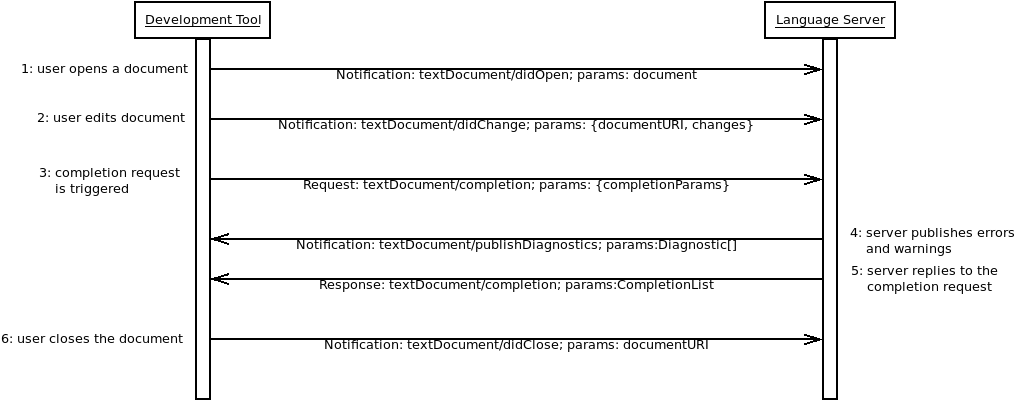
\includegraphics[width=\textwidth]{lsp.png}
	\caption{Sequence Diagram LSP}
	\label{seqDiagLSP}
\end{figure}

\begin{enumerate}
	\item \textbf{The user opens a file (referred as a \textit{document})}: the tool notifies the server that a document is open (\verb|textDocument/didOpen|), meaning that it is kept in the tool memory. The server will therefore save the language representation of the document in its memory.
	\item \textbf{The user edits the document}: the tool notifies the server about a change made by the user on the document (\verb|textDocument/didChange|). The server updates the language representation of the document.
	\item \textbf{The tool execute the Completion Request}: the request (\verb|textDocument/completion|) is triggered right after the \verb|textDocument/didChange|. The parameter, \textit{completionParams}, is essentially a JSON object with all the necessary information (documentURI, position, triggerKind) that the server needs to compute the response. Note that this call is \textit{asynchronous}: the tool can send other notifications or request while waiting for the completion response, correspondingly the LS can answer asynchronously.
	\item \textbf{The server publishes errors and warnings}: after the change notification, the server computes and notifies the tool with a list of eventual errors and warnings in the code\\(\verb|textDocument/publishDiagnostics|). The parameters of this notification contains all the necessary information in order to permit the tool flags errors and warnings.
	\item \textbf{The server replies to the Completion Request}: the server after computing a list of possible completion items, replies to the completion request made before by the tool. The latter lists the items received in order to let the user decide which suites the best.
	\item \textbf{The user closes the document}: the tool notifies the server when the user closes the document, which cease to exist in the tool memory. The server erases all the information regarding the document. 
\end{enumerate}

All the data types illustrated are language agnostic, meaning that can be applied to all the programming languages. This is due to the protocol simplicity: it is simpler to standardize a document URI or a position inside a it, than standardizing an \textit{Abstract Syntax Tree} and compiler symbol across different programming languages.\\This simplicity is shown in the following JSON-RPC objects that refers to the completion request and response:

\textbf{Request}
\begin{lstlisting}[language=json]
{
	"jsonrpc": "2.0",
	"id" : 1,
	"method": "textDocument/completion",
	"params": {
		"textDocument": {
			"uri": "file:///home/user/Desktop/client.ol"
		},
		"position": {
			"line": 3,
			"character": 7
		},
		"context": {
			"triggerKind": 1
		}
	}
}
\end{lstlisting}

\textbf{Response}
\begin{lstlisting}[language=json]
{
	"jsonrpc": "2.0",
	"id": 1,
	"result": {
	"isIncomplete": false,
		"items": {
			"label": "println@Console",
			"kind": 2,
			"insertText": "println@Console( $1 )( $2 )",
			"insertTextFormat": 2
		}
	}
}
\end{lstlisting}

A LS in order to work with LSP does not need to implement all the features. LSP provides \textbf{capabilities}. A capability groups a set of language features. The protocol permits the server to notify the tool which capabilities supports, therefore the tool adapts itself in order to send notifications and requests of the supported capabilities.
\subsection{Server Protocol features}
LSP supports six key features which are:
\begin{enumerate}
	\item \textbf{Code completion}: feature that speeds up the process of coding applications by reducing typos and other common mistakes;
	\item \textbf{Hover information}: feature that shows information, like the type signature, when the user moves the pointer over an element (such as a function definition);
	\item \textbf{Jump to definition}: feature that shows the definition of a selected symbol;
	\item \textbf{Workspace symbols}: displays all the symbols of the workspace, in order to help the user search for elements inside the workspace (such as classes, variables, methods, etc.);
	\item \textbf{Find references}: given a symbol, this features lists all the project wide references;
	\item \textbf{Diagnostics}: the tool flags syntax errors, warnings together with a description.
\end{enumerate}
The protocol supports many other features that are all linked to these ones. The requirements elicitation phase was based on these main ones.
\chapter{Analysis of the problem}
\label{sec:Analysis}
In this Chapter we will identify the requirements, gathered during the analysis of the Language Server Protocol and over a series of meetings with the supervisor.
\section{Functional Requirements}
\label{sec:FR}
Functional requirements are statements of services the system should provide, particularly how it should react to particular inputs \cite{Som11}. From the features analyzed in the previous section, we extracted eight functional requirements, which  are listed in Table \ref{FRCpt3} in descending order of importance.
\begin{table}[t]
	\caption{Functional Requirements}
	\begin{tabularx}{\textwidth}{c|X}
		\hline
		\textbf{Functional r. No.} & \textbf{Description}\\
		\hline\hline
		FR 1 & The server must provide information of eventual programming errors and warnings every time a document is opened/modified.\\\hline
		FR 2 & Every time the user starts typing an operation name, the server returns a list of possible completion items that consists of the full operation name and the output port.\\\hline
		FR 3 & Every time the user starts typing a keyword, the server provides a list of possible completion items.\\\hline
		FR 4 & Every time a document is opened/modified/closed, the server saves/updates/deletes the information in his memory like the text, URI and a data structure containing all the information regarding the Jolie program (an Abstract Syntax Tree of the \textit{behavior} and data regarding the \textit{deployment}).\\\hline
		FR 5 & The server provides the type signature to the client every time the latter sends an hover request.\\\hline
		FR 6 & The server provides a list or hierarchy of symbols of a specific document requested by the client.\\\hline
		FR 7 & The server computes and sends the operation definition every time it receives a definition request\\\hline
		%FR 8 & Information regarding the workspace are sent to the client and updated every time the client requests them (workspace symbols for example).\\\hline
		FR 8 & The server resolves project wide references of a given symbol.\\\hline 
	\end{tabularx}
	\label{FRCpt3}
\end{table}

\section{Non-functional requirements}
\label{sec:NFR}
Non-functional requirements are requirements that are not directly concerned with the specific services delivered by the system to its users. They may relate to emergent system properties such as reliability, response time, and store occupancy. Alternatively, they may define constraints on the system implementation such as the capabilities of I/O devices or the data representations used in interfaces with other systems \cite{Som11}.

Regarding our project, the response time is critical, as the server should be able to respond to the client as soon as possible. Nonetheless, this kind of calculations (such as code completion) are not computationally heavy. Other non-functional requirements, are listed below, while the complete list can be sees at Table \ref{NFRCpt3}.
\begin{table}[t]
	\caption{Non-Functional Requirements}
	\begin{tabularx}{\textwidth}{c|X}
		\hline
		\textbf{Non-functional r. No.} & \textbf{Description}\\
		\hline\hline
		NFR 1 & The server must support the LSP's JSON-RPC protocol.\\\hline
		NFR 2 & The server must be designed to be modular.\\\hline
		NFR 3 & The server must be able to respond to a client request as soon as possible.\\\hline
		NFR 4 & The server must work both when deployed in a different machine and when deployed in a local machine, with respect of the client location. As a consequence, it has to support the socket channel of communication.\\\hline
		NFR 5 & The server must be able to handle more clients sending multiple requests concurrently.\\\hline
	\end{tabularx}
	\label{NFRCpt3}
\end{table}
\subsection{Complying with the Language Server Protocol specification}
The Language Server Protocol defines a common language, between a tool and a Language Server. As a consequence, the latter must be able to recognize different requests received from the client and send back proper responses that the client is able to interpret and compute.

Following an example: the request-response method \verb|initialize|, that provides the server client's capabilities and it expects a response with the server capabilities, has the following type:
\clearpage
\textbf{Request type}
\begin{lstlisting}[language=javascript]
interface InitializeParams {
	processId: number | null;
	rootPath?: string | null;
	rootUri: DocumentUri | null;
	initializationOptions?: any;
	capabilities: ClientCapabilities;
	trace?: 'off' | 'messages' | 'verbose';
	workspaceFolders?: WorkspaceFolder[] | null;
}
\end{lstlisting}

\textbf{Response type}
\begin{lstlisting}[language=javascript]
interface InitializeResult {
	/**
	 * The capabilities the language server provides.
	 */
	capabilities: ServerCapabilities;
}
\end{lstlisting}
\subsubsection{JSON-RPC 2.0 Protocol}
Regarding the communication protocol, LSP supports a custom version of the JSON-RPC 2.0 protocol, as mentioned in \hyperref[sec:JolieLSP]{Chapter 2}. A message is characterized by an header part, which can contain up to two headers (Content-Length, which is mandatory, and Content-Type) and a content part, with the actual message represented with the JSON-RPC notation.

Jolie supports JSON-RPC, but it runs over HTTP, therefore Jolie's JSON-RPC will expect HTTP headers before the Content-Length and Content-Type. As a consequence, Jolie's JSON-RPC protocol must be extended in order to make it compatible with LSP messages.
\subsection{Distributed architecture}
The server must be adapted to the LSP, in order to make it work with different tools that use the protocol concerned. Therefore, it must be \textbf{editor-agnostic} and it should be designed and implemented in order to be deployed both locally and in a different machine with respect to the clients, so it can interact with different tools, at the same time. %The LSP specifications indicate that when the development tool starts the plug-in, the latter will immediately start.
 Consequently the best communication channel to use is the TCP socket, in order to guarantee the platform independence.
\subsection{Modularity}
Not every LS can support all features defined by the protocol. LSP therefore provides, the previous mentioned, \textbf{capabilities}, as stated in \hyperref[sec:JolieLSP]{Chapter 2}. A capability groups a set of language features. A development tool and the LS announces their supported features using capabilities. For instance, the server announces that it can handle the \verb|textDocument/hover| request, but it might not support the \verb|textDocument/references| request. Similarly, a development tool announces its ability to provide \verb|textDocument/didChange| notification when a document is modified, so that a server can compute textual edits to format the edited document. On account of this, the server must be designed in order to easily add new capabilities or improve the existing ones. After implementing a new feature, the programmer just need to modify the server capabilities thus the client can start sending requests regarding the newly activated capability.
\chapter{System architecture}
\label{sec:arch}
The architecture of a system identifies the components that form a system and the relationships between them. Graphical models are the best technique to abstractly represent a system architecture. Software architecture is important because it affects the performance, robustness,
distributability and maintainability of a system \cite{Bosch:2000:DUS:339362}. In order to satisfy the non-functional, in particular \hyperref[sec:NFR]{NFR 2} and \hyperref[sec:NFR]{NFR 5} requirements defined in \hyperref[sec:Analysis]{Chapter 3}, we adopt the Service Oriented Architecture (SOA). Instead of a monolithic architecture, SOA is more scalable: the direct communication with the client is handled by a single service which deals with the initialization and the termination of the entire server while it forwards all the other requests and notifications sent by the development tool to the service responsible for treating the specific message (e.g. the message \verb|textDocument/didOpen|, when received by the main service, named \textit{orchestrator}, forwards the message to the textDocument service, namely the service that handles all the textDocument messages).
\section{Architecture}
In this section we will see two architectures according to NFR 4. One architecture, represents the system with the LS deployed in the same machine as the development tool, while the other describes the architecture of the system when the LS is deployed in a different machine than the client. The hexagon represents a \textit{macroservice}, which is an unique execution context for a set of services. A macroservice exhibits only the public available ports of the inner services \cite{JolieDoc}.

The distributed architecture shows that the single LS is capable of serving more clients concurrently, however this could be implemented also in a single machine, having a single LS running that serves one or more editors. This requires the use of a \emph{Proxy Service} which is spawned directly by the client, as the latter expects a child process containing the server. The local architecture presented, at the contrary, expects that there is more than one instance of the LS, namely for each different client opened a LS program is spawned, therefore there is no need for the proxy. 

The LS is \emph{stateful}, meaning that it keeps track of the state of interaction. In particular, the state is kept in memory and it is \emph{transient}. This means that if for some reason the LS terminates its execution, the state is lost. This implies that, in the distributed model, the LS must be able to distinguish which client the information kept belongs to by using \emph{sessions}, which must be handled in parallel.

\begin{figure}[t]
	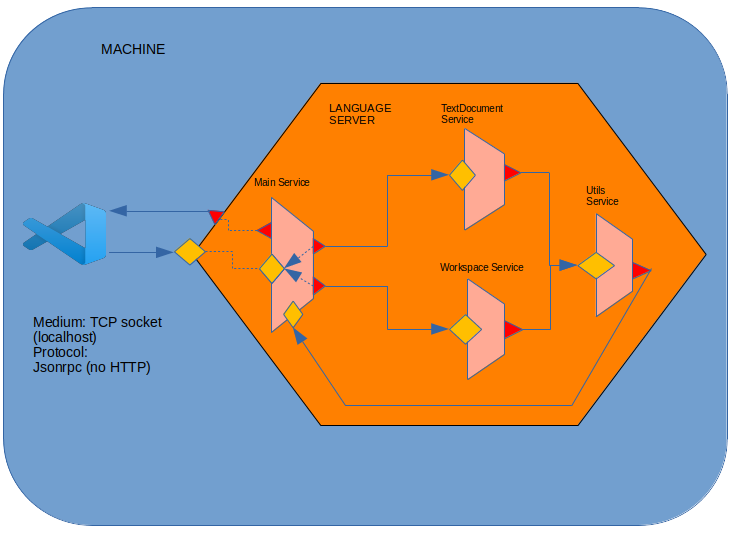
\includegraphics[width=\textwidth]{local_arch.png}
	\caption{Architecture in L.S. and dev. tool in a single machine}
	\label{localArch}
\end{figure}
\begin{figure}[t]
	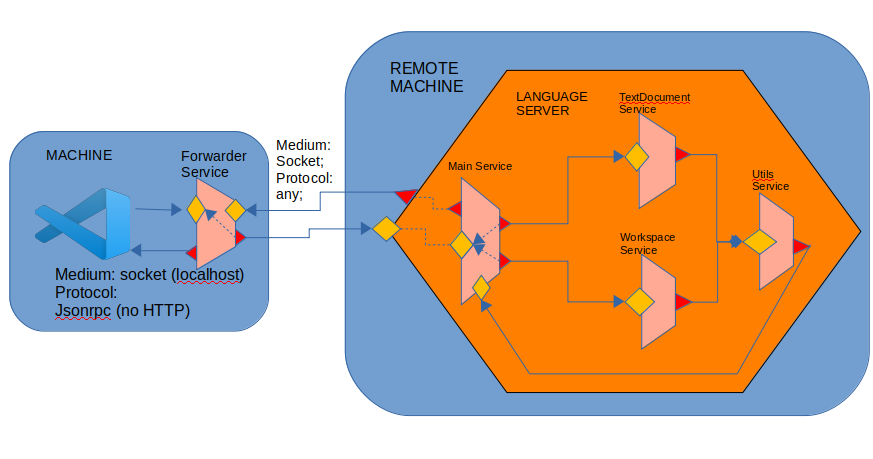
\includegraphics[width=\textwidth]{distr_arch.png}
	\caption{L.S. and dev. tool in different machines}
	\label{distrArch}
\end{figure}
\begin{figure}[t]
	\centering
	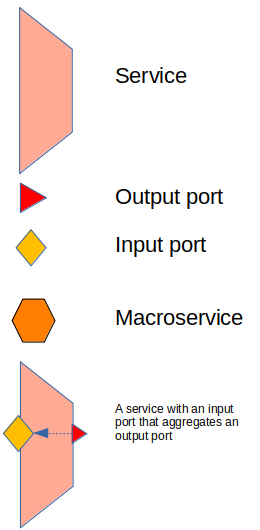
\includegraphics[height=10cm]{legenda.png}
	\caption{Legenda}
	\label{legenda}
\end{figure}


\section{Services}
Each service presented in the model has a set of operations which will be briefly described in this section.
\subsection{Main service}
The main service presents two input ports and three output ports. One input port is used to receive the requests and notifications sent by the client, the other is used by another service, called \textbf{utils}, with the purpose to receive all the notifications to be sent to the client through one of the output ports. The remaining two output ports point to the two main services of the server, \textbf{textDocument} and \textbf{workspace} and they should be aggregated by the first mentioned input port, therefore every message is automatically forwarded to the respective service.

The operations offered by this service are necessary for initialization and termination of the server. For more details see \cite{LSPSpec}. The service must handle at least the following requests and notifications:
\begin{itemize}
	\item \verb|initialize| request which content contains the \textit{client capabilities}. The response consists of the \textit{server capabilities}. In the distributed model, this is where a session is started: the proxy, after receiving the initialize request, communicates with the LS, which it will start a new session and reply with the server capabilities;
	\item \verb|initialized| notification. An empty message acting as an ACK for the \verb|initialize| response;
	\item \verb|shutdown| request. Empty message that expects an empty response. In the distributed model, the proxy, before sending the empty response, sends a notification to the LS in order to close the session;
	\item \verb|exit| notification. After receiving the \verb|shutdown| response, a notification is sent and the server or the proxy must terminate its execution.	
\end{itemize}
\subsection{Text Document service}
The service \emph{textDocument} handles all the text document messages. In order to meet the \hyperref[sec:FR]{functional requirements} the service must serve the following messages:
\begin{itemize}
	\item \verb|textDocument/completion| request. This request is sent with a cursor position and expects a response with a list of completion items that will be presented in the user interface;
	\item \verb|textDocument/didOpen|, \verb|textDocument/didChange|, \verb|textDocument/didClose| notifications. Messages used for synchronizing the document's truth with the language server. The service should forward the message to the service \textbf{utils} that will respectively store, update or delete the information regarding the document (URI, text, etc.);
	\item \verb|textDocument/hover| request is sent together with a cursor position thus the service could compute a response with the information of what is located in that document position.
	\item \verb|textDocument/documentSymbol| request requires a flat list or hierarchy of symbols of a specified document.
	\item \verb|textDocument/definition| request. The client requires the server to resolve the definition location of a given document symbol at a given text document position.
	\item \verb|textDocument/references| request is sent in order to resolve project-wide reference of the symbol denoted by the given text document position.
\end{itemize}
For all the text document messages, see \cite{LSPSpec}.
\subsection{Workspace service}
All the workspace messages are handled by this service. More details regarding this type of messages can be studied at \cite{LSPSpec}.
\subsection{Utils service}
\emph{Utils} service provides functionalities such as syntax checking and document synchronization. For each time a document synchronization message, e.g. \verb|textDocument/didChange|, is received by \emph{textDocument} service, the latter forwards it to \emph{Utils} service that keeps a data structure with all the documents that are open in a specific moment. Subsequently, a syntax check is executed on the updated or newly opened document and the result is sent to the main service which in turn forwards it to the client.
\subsection{Proxy service}
The \emph{Proxy Service} is an additional service used for the distributed system. The input port exposed to the development tool aggregates the output port used for contacting the server. Jolie is \emph{protocol agnostic}. This means that the communication between the proxy and the Language Server does not need to use the JSON-RPC protocol: the aggregator, which in our case is the proxy, automatically transforms the messages thus granting a transparent composition of the server.
\chapter{Implementation}
\label{sec:impl}
For implementing the Language Server for Jolie, modeled in the previous Chapter, we used the language Jolie itself for the following reasons:
\begin{itemize}
	\item \textbf{Service orientation}: Jolie, as described in \hyperref[sec:JolieLSP]{Chapter 2}, is microservice-oriented language, which is perfect for the non-functional requirements described in \hyperref[sec:Analysis]{Chapter 3}, in particular NFR 1, as Jolie already supports the JSON-RPC protocol over HTTP, therefore it must be adapted to the protocol used by LSP, in order to recognize LSP messages and parse them properly. This required the implementation of a parser able to parse LSP headers correctly and pass the actual JSON message to the already existing parsing libraries, converting a JSON string into a Jolie Value (and vice versa). Moreover, Jolie has a service included in the standard library, called \emph{Inspector}, that provides code inspection operations for analyzing Jolie source code, therefore useful in order to meet \hyperref[sec:FR]{FR 1} and \hyperref[sec:FR]{FR 2}.
	\item The macroservice concept is realized with the \emph{static embedding} primitive: the main service embeds all the other three services, therefore all four services will run in the same virtual machine. This will reflect in faster internal communications. Furthermore, the main service \emph{aggregates} the output ports pointed respectively to the services \emph{workspace} and \emph{textDocument} to guarantee an automatic forward of the messages that are not of its concern.
\end{itemize}
The implementation phase was based on the local architecture model described in the previous Chapter and it was characterized by the following two steps:
\begin{enumerate}
	\item \textbf{Complying with the LSP's JSON-RPC specifications}: LSP uses a simplified version of JSON-RPC protocol, whereas Jolie internal JSON-RPC protocol uses it over HTTP. Therefore, the protocol was extended in order to be capable of handling also LSP messages. Moreover, the Jolie interpreter, when receiving a JSON-RPC message is able to redirect it to the correct operation by using the \emph{method} field in the JSON-RPC message. Despite this, most of the method names in LSP have prefixes, for instance \verb|textDocument/didOpen|, which is problematic as operation names in Jolie does not support special characters such as the \say{/}. As a consequence, Jolie's protocol must be extended in order to alias the operation names properly. 
	\item \textbf{Implementation of the Language Server}: define all the services with their deployment parts (ports, types and interfaces) and their behavior (computations).
\end{enumerate}
\section{Complying with LSP JSON-RPC specifications}
\subsection{LSP message and parser}
In order to extend Jolie JSON-RPC protocol, \emph{protocol parameters} were exploited. Input port protocol definitions could be extended with parameters, namely a list of options regarding compression, debug settings, etc.. The parameter added, called \emph{transport} is a simple string. Following an example of an input port using JSON-RPC with the parameter described above.
\begin{lstlisting}[language=Jolie]
	inputPort Input {
		location:JolieLS
		protocol: jsonrpc {
			transport = "lsp"
		}
		interfaces:...
		...		
		}
\end{lstlisting}

Jolie, when it identifies this parameter, must not use JSON-RPC over HTTP, but according to LSP specification. In order to do this, the modifications made in the Jolie protocol are:
\begin{itemize}
	\item Definition of two new classes: \verb|LSPMessage| and \verb|LSPParser|. The first represents an LSP message, according to the specifications defined in \hyperref[sec:JolieLSP]{Chapter 2}, the second is a parser used on the data read from the buffer, in order to extract headers and the JSON object properly, therefore, the latter is parsed by the \verb|JsUtils| class in order to obtain a Jolie value representation of the original JSON message.
	\item Modified \verb|JsonRpcProtocol| class definition which now checks if there is the parameter \emph{transport} with value \verb|"lsp"|, and, according to the result of this check, uses the appropriate parser (HTTP or LSP).
\end{itemize}

Following the \verb|LSPMessage| class definition:
\begin{lstlisting}[language=java]
	public class LSPMessage {
		
    	private byte[] content = null;
    	final private Map< String, String > propMap = new HashMap<>();

    	public String getProperty( String name ) {
        	String property = getPropMap().get( name.toLowerCase() );
        	if(property!=null)
            	property=property.trim();
        	return property;
    	}

    	protected Map<String, String > getPropMap() {
        	return propMap;
    	}
    	public void setContent( byte[] content ) {
        	this.content = content;
    	}

    	public void setProperty(String name, String value) {
        	propMap.put( name.toLowerCase(), value );
    	}

    	public Collection< Entry< String, String > > getProperties() {
        	return propMap.entrySet();
    	}

    	public int size() {
        	if ( content == null )
            	return 0;
        	return content.length;
    	}

    	public byte[] content() {
        	return content;
    	}
	}
\end{lstlisting}
where the field \verb|content| represents the JSON message, while \verb|propMap| is an \verb|HashMap| containing the header names and their relative values.
\subsection{Aliasing LSP method names to Jolie operation names}
Similarly to the problem presented in the previous section, aliasing must be handled at protocol level. Therefore we used the parameter \verb|osc|, acronym for \emph{operation specific parameter}, for each operation name to be aliased.
\begin{lstlisting}[language=Jolie]
	inputPort Input {
		location:JolieLS
		protocol: jsonrpc {
			transport = "lsp"
			osc.didOpen.alias = "textDocument/didOpen"
			osc.didClose.alias = "textDocument/didClose"
			osc.completion.alias = "textDocument/completion"
			...
		}
		interfaces:...
		...		
	}
\end{lstlisting}

The above example demonstrate that protocol parameter is a Jolie \emph{data tree}. The parameter \verb|osc| must have a child node with the name of the operation and in turn a child node name \verb|alias| with a string value that represents the alias.

The modifications made in the \verb|JsonRpcProtocol| class were substantially the following:
\begin{itemize}
	\item When \textbf{receiving} a message, after the parsing phase, given the LSP method name contained in the subnode \verb|method|, compute the correspondent operation name in the Jolie program, by visiting the \verb|osc| tree.
	\item When \textbf{sending} a message, the steps are analogue, but the aliasing is done before parsing the Jolie value to a JSON string and it is from the Jolie operation name to the LSP method name.
\end{itemize}
Following the code for aliasing operation names when receiving a message.
\begin{lstlisting}[language=java]
	String operation = value.getFirstChild( "method" ).strValue();
                        
	// Resolving aliases
	if ( hasParameter( Parameters.OSC ) ) {
		Value osc = getParameterFirstValue( Parameters.OSC );
		for( Entry<String, ValueVector> ev : osc.children().entrySet() ) {
			Value v = ev.getValue().get( 0 );
			if ( v.hasChildren( Parameters.ALIAS ) ) {
				if ( v.getFirstChild( Parameters.ALIAS ).strValue().equals( operation ) ) {
					operation = ev.getKey();
				}
			}
		}
	}
\end{lstlisting}

The variable \textcolor{color:keyword}{operation} contains the name of the LSP method name (e.g. \verb|textDocument/didOpen|), the variable \textcolor{color:keyword}{osc} is the root of the data tree. \textcolor{color:keyword}{Value} and \textcolor{color:keyword}{ValueVector} are the classes used to represent data trees in Jolie. Each single node of a tree in Jolie is a \textcolor{color:keyword}{ValueVector} containing one or more objects of type \textcolor{color:keyword}{Value} which contains basic type value and its children nodes, which in turn are \textcolor{color:keyword}{ValueVector} objects. The code for aliasing an outgoing message is analogue.
\begin{lstlisting}[language=java]
	String operationNameAliased = message.operationName();
		//resolving aliases
	if ( hasParameter( Parameters.OSC ) ) {
		Value osc = getParameterFirstValue( Parameters.OSC );
		for( Entry<String, ValueVector> ev : osc.children().entrySet() ) {
			Value v = ev.getValue().get( 0 );
			if ( v.hasChildren( Parameters.ALIAS ) ) {
				if ( ev.getKey().equals( operationNameAliased ) ) {
					operationNameAliased = v.getFirstChild( Parameters.ALIAS ).strValue();
				}
			}
		}
	}
\end{lstlisting}
\subsection{Improvements for Jolie's jsonrpc protocol}
JsonRpcProtocol class avails of a utility library, named \verb|jolie.js.JsUtils|, which provides functionalities to convert Jolie values to JSON strings and vice versa. Namely, the method\\\verb|valueToJsonString(Value value, boolean extendedRoot, Type type, StringBuilder builder)|, given a Jolie value, the type of the value and a \verb|StringBuilder|, generates a JSON string and saves it in the last mentioned argument.\\ The third argument of type \verb|Type|, which, in the Jolie interpreter, represents the full type description of a Jolie message, could accept either an \verb|undefined| type and, in this situation, the method is able to perform its task by using the structure of the first argument, or a type, obtained by the interfaces of the Jolie program. When passing \verb|undefined|, the conversion is not \emph{strict}. Following an example showing the the input an output with argument type as \verb|undefined|. Given the following type of a Jolie value
\begin{lstlisting}[language=jolie]
	type T_root {
		node[1,*]: int
	}
\end{lstlisting}
and a value of the above type
\begin{lstlisting}[language=jolie]
	v << {
		node = 1
	}
\end{lstlisting}
the following JSON string is obtained
\begin{lstlisting}[language=json]
	{
		"node" : 1
	}
\end{lstlisting}
while, if the type above described is passed to the method, the result is the following.
\begin{lstlisting}[language=json]
	{
		"node": [1]	
	}
\end{lstlisting}
This behavior is due to the fact that the parser will set \verb|"node"| as an array only if there are at least two elements in the Jolie node. Therefore in order to force the parser to produce the last result listed, the type of the value must be passed as an argument to the method.\\The implementation of the JSON-RPC protocol in Jolie was \emph{always} passing an \verb|undefined| type to the method, despite the Jolie value had a defined type structure in an interface. The fix consisted in extracting the type of the message from the interfaces present in the communication port of the program, and, if present, we pass it to the \verb|valueToJsonString| method, otherwise we pass the type \textcolor{color:keyword}{undefined}.
\section{Server implementation}
The server structure is the presented in \hyperref[sec:arch]{Chapter 4}, thus it will be composed by four Jolie programs together with the files containing respectively the types definitions and the interfaces used by the various ports. The full implementation of the server can be viewed at the reference \cite{JolieLangSupport}.
\subsection{Operation types and interfaces}
Though Jolie operations can have type \textcolor{color:keyword}{undefined}, all the operation types have been defined accordingly to the LSP specification, in order to type check every message to be received and sent. Therefore, \textbf{maintainability} will be affected positively, as changes in the type definitions of LSP messages that might be applied in future releases of the protocol, can be identified immediately as the type check could fail, sending a fault to the invoker or to the server itself. Following the interface definitions for all the ports used in the service.
\begin{lstlisting}[language=Jolie]
	include "types/lsp.iol"

	interface GeneralInterface {
  		OneWay:
    		initialized( InitializedParams ),
    		onExit( void ),
    		cancelRequest //cancelRequest( undefined )
  		RequestResponse:
    		initialize( InitializeParams )( InitializeResult ),
    		shutdown( void )( void )
	}

	interface TextDocumentInterface {
  		OneWay:
    		didOpen( DidOpenTextDocumentParams ),
    		didChange( DidChangeTextDocumentParams ),
    		willSave( WillSaveTextDocumentParams ),
    		didSave( DidSaveTextDocumentParams ),
    		didClose( DidCloseTextDocumentParams )
  		RequestResponse:
    		willSaveWaitUntil( WillSaveTextDocumentParams )( WillSaveWaitUntilResponse ),
    		completion( CompletionParams )( CompletionResult ),
    		hover( TextDocumentPositionParams )( HoverInformations ),
    		documentSymbol( DocumentSymbolParams )( DocumentSymbolResult ),
    		signatureHelp( TextDocumentPositionParams )( SignatureHelpResponse )
	}

	interface WorkspaceInterface {
  		OneWay:
    		didChangeWatchedFiles( DidChangeWatchedFilesParams ),
    		didChangeWorkspaceFolders( DidChangeWorkspaceFoldersParams ),
    		didChangeConfiguration( DidChangeConfigurationParams )
  		RequestResponse:
    		symbol( WorkspaceSymbolParams )( undefined ),
    		executeCommand( ExecuteCommandParams )( ExecuteCommandResult )
	}

	interface ServerToClient {
  		OneWay:
    		publishDiagnostics( PublishDiagnosticParams )
	}

	interface UtilsInterface {
  		RequestResponse:
    		getDocument( string )( TextDocument )
  		OneWay:
    		insertNewDocument( DidOpenTextDocumentParams ),
    		updateDocument( DocumentModifications ),
    		deleteDocument( DidCloseTextDocumentParams )
	}

\end{lstlisting}
The full type definitions can be viewed at the reference \cite{LSPSpec}.
\subsection{Main service}
The main service handles the initialization and termination of the server. Furthermore it \emph{orchestrates} the messages sent by the development tool to the services that are concerned.
\begin{lstlisting}[language=Jolie]
	/*
 	 * Main Service that communicates directly with the client and provides the basic
 	 * operations
	 */
	execution { sequential }

	include "internal/deployment.iol"

	include "console.iol"
	include "string_utils.iol"
	include "runtime.iol"

	init {
  		Client.location -> global.clientLocation
  		println@Console( "Jolie Language Server started" )()
  		global.receivedShutdownReq = false
	}

	main {
    	[ initialize( initializeParams )( serverCapabilities ) {
      		println@Console( "Initialize message received" )()
      		global.processId = initializeParams.processId
      		global.rootUri = initializeParams.rootUri
      		global.clientCapabilities << initializeParams.capabilities
      		//for full serverCapabilities spec, see
      		// https://microsoft.github.io/language-server-protocol/specification
      		// and types.iol
      		serverCapabilities.capabilities << {
        		textDocumentSync = 1 //0 = none, 1 = full, 2 = incremental
        		completionProvider << {
          		resolveProvider = false
          		triggerCharacters[0] = "@"
        		}
        		//signatureHelpProvider.triggerCharacters[0] = "("
        		definitionProvider = false
        		hoverProvider = true
        		documentSymbolProvider = false
        		referenceProvider = false
        		//experimental;
      		}
    	} ]

    	[ initialized( initializedParams ) ] {
      		println@Console( "Initialization done " )()
    	}

    	[ shutdown( req )( res ) {
        	println@Console( "Shutdown request received..." )()
        	global.receivedShutdownReq = true
    	} ]

    	[ onExit( notification ) ] {
      		if( !global.receivedShutdownReq ) {
        		println@Console( "Did not receive the shutdown request, exiting anyway..." )()
      		}
      		println@Console( "Exiting Jolie Language server..." )()
      		exit
    	}
    	//received from utils.ol
    	[ publishDiagnostics( diagnosticParams ) ] {
      		println@Console( "publishing diagnostics for " + diagnosticParams.uri )()
      		publishDiagnostics@Client( diagnosticParams )
    	}

    	[ cancelRequest( cancelReq ) ] {
        	println@Console( "cancelRequest received ID: " + cancelReq.id )()
        	//TODO
    	}
	}
\end{lstlisting}
The \emph{deployment} part of this service is imported from another file with the primitive \textcolor{color:keyword}{include}. The \emph{behavior} is an input choice, in which initialization and termination of the server are handled. When the service receives an \verb|initialize| message, it executes the behavior of the input \emph{initialize} where the client capabilities are saved in a data structure and the \verb|serverCapabilities| are computed and sent to the invoker. Consequently, the client, after receiving the language server capabilities it sends an \verb|initilized| notification with no content and the interaction can start. \textbf{Termination} follows the same steps: first, the client send an empty \verb|shutdown| request, and after receiving the response, it sends a \emph{exit} notification, aliased to \verb|onExit|, as \textcolor{color:keyword}{exit} is a reserved word, where the server must terminate its execution.
\subsection{Utils service}
Utils service has four input operations:
\begin{itemize}
	\item \textbf{insertNewDocument}: after receiving a \verb|textDocument/didOpen| message from the development tool, the document received is inspected through the \emph{Inspector} service, which extracts information like output and input ports, their interfaces with the operation definitions and the type definition of the latters. Nonetheless, if there is a syntax error in the document received, the \emph{Inspector} provides a string containing all the information related to this error, including the position. This is used two build a \verb|diagnosticParam| structure to be sent to the main service previously described, which in turn forwards it to the client. When the latter receives the diagnostics, it will publish them through its UI. If the document does not have any error, the document data, namely the \emph{uri}, the \emph{source code}, the \emph{inspection result} and an array containing the lines of code, are saved normally in a global variable. This variable is an array containing all the documents that are opened in the development tool.
	\item \textbf{updateDocument}: the message received through the notification \verb|textDocument/didChange| is forwarded to this input operation, that similarly achieves what \verb|insertDocument| does. Unlikely the latter, \verb|updateDocument| publishes also the empty diagnostics, in order to clear the client's UI when a syntax error is corrected by the user.
	\item \textbf{deleteDocument}: input operation that receives a document URI and deletes the array element containing the correspondent URI.
	\item \textbf{getDocument}: request-response operation that sends to the invoker the full data structure with the corresponding URI received. This operation is used by Text Document service in order to perform tasks like \verb|completion| and \verb|hover|.
\end{itemize}
\subsection{Text Document service}
The purpose of this service is to handles all the text document messages sent by the development tool, for instance \verb|textDocument/didOpen| or \verb|textDocument/completion|. Two main features has been implemented: \textbf{auto-completion} for operation definitions and keywords, and \textbf{hover} information of both input and output operation definitions.
\subsubsection{Completion}
Given a text document position, the server ought to compute a list of possible completion item to integrate what is already present in that document position. We implemented this functionality for auto-completing output statements. For instance, if in the given text document position the server finds "pri", it ought to compute a list of output operations that are found in the interfaces of the output ports of the service. In this case, the server will return the following list: \texttt{["print@Console( \$1 )( \$2 )", "println@Console( \$1 )( \$2 )"]}. These completion items are in the form of \textbf{snippets}. A \textbf{snippet} is a small and reusable piece of code, in which tab stops and placeholders can be defined with the \texttt{\$1}, \texttt{\$2} and \texttt{\$\{3:foo\}}. \texttt{\$0} identifies the end of the snippet. Placeholders with equal identifiers are linked, that is typing in one will update the others too \cite{LSPSpec}.\\Following the code of the \verb|completion| input operation.
\begin{lstlisting}[language=Jolie]
	/*
   * RR sent sent from the client when requesting a completion
   * works for anything callable
   * @Request: CompletionParams, see types/lsp.iol
   * @Response: CompletionResult, see types/lsp.iol
   */
  [ completion( completionParams )( completionRes ) {
      println@Console( "Completion Req Received" )()
      completionRes.isIncomplete = false
      txtDocUri -> completionParams.textDocument.uri
      position -> completionParams.position

      if ( is_defined( completionParams.context ) ) {
        triggerChar -> completionParams.context.triggerCharacter
      }

      getDocument@Utils( txtDocUri )( document )
      //character that triggered the completion (@)
      //might be not defined

      program -> document.jolieProgram
      codeLine = document.lines[position.line]
      trim@StringUtils( codeLine )( codeLineTrimmed )
      portFound = false
      
      for ( port in program.outputPorts ) {
        for ( iFace in port.interfaces ) {
          for ( op in iFace.operations ) {
            if ( !is_defined( triggerChar ) ) {
              //was not '@' to trigger the completion
              contains@StringUtils( op.name {
                substring = codeLineTrimmed
              } )( operationFound ) // TODO: fuzzy search
              undef( temp )
              if ( operationFound ) {
                snippet = op.name + "@" + port.name
                label = snippet
                kind = CompletionItemKind_Method
              }
            } else {
              //@ triggered the completion
              operationFound = ( op.name == codeLineTrimmed )

              label = port.name
              snippet = label
              kind = CompletionItemKind_Class
            }

            if ( operationFound ) {
              //build the rest of the snippet to be sent
              if ( is_defined( op.responseType ) ) {
                //is a reqRes operation
                reqVar = op.requestType.name
                
                resVar = op.responseType.name
                if ( resVar == NATIVE_TYPE_VOID ) {
                  resVar = ""
                }
                snippet += "( ${1:" + reqVar + "} )( ${2:" + resVar + "} )"
              } else {
                //is a OneWay operation
                notificationVar = op.requestType.name
                
                snippet = "( ${1:" + notificationVar + "} )"
              }

              //build the completionItem
              portFound = true
              completionItem << {
                label = label
                kind = kind
                insertTextFormat = 2
                insertText = snippet
              }
              completionRes.items[#completionRes.items] << completionItem
            }
          }
        }
      }

      //loop for completing reservedWords completion
      keyword -> global.keywordSnippets
      for ( i=0, i<#keyword.snippet, i++ ) {
        contains@StringUtils( keyword.snippet[i] {
          substring = codeLineTrimmed
        } )( keywordFound )

        if ( keywordFound ) {
          completionItem << {
            label = keyword.snippet[i]
            kind = CompletionItemKind_Keyword
            insertTextFormat = 2
            insertText = keyword.snippet[i].body
          }
          completionRes.items[#completionRes.items] << completionItem
        }
      }
      
      if ( !foundPort && !keywordFound ) {
        completionRes.items = void
      }
      println@Console( "Sending completion Item to the client" )()
  } ]
\end{lstlisting}
Given the text document URI and the text document position, it retrieves the text document by sending a \verb|getDocument| message to the Utils service, thus extracts the code line of interest (lines 9-24). Subsequently, it traverses all the operations in each interface for each output port present in the program and, for each matching element found, a snippet is built and inserted in the response to be sent (lines 26-79). Afterwards, the same search is done inside a data structure containing the keywords' snippets (lines 82-97). If nothing is found, an empty array is sent to the invoker (lines 99-101).\\
Let $n$ be the number of operations defined in all the output ports present in the program. Let $m$ be the number of elements in the array containing the keywords' snippets. The complexity of this algorithm is therefore $T(n,m) = O(n)+O(m)$. Though, the number of keywords is constant therefore the time complexity is $T(n) = O(n)$. In order to improve performance in terms of execution time, Jolie parallel constructs could have been used, namely perform a parallel search for each output port. However, this solution is not convenient as Jolie interpreter would spawn a determinant number of threads and, since in a program there would not be more than a hundred operations to be searched, using the sequential linear search is the simplest solution.
\subsubsection{Hover}
The hover request-response operation works similarly to the previously explained.
\begin{lstlisting}[language=jolie]
  /*
   * RR sent sent from the client when requesting a hover
   * @Request: TextDocumentPositionParams, see types.iol
   * @Response: HoverResult, see types.iol
   */
  [ hover( hoverReq )( hoverResp ) {
    found = false
    println@Console( "hover req received.." )()
    textDocUri -> hoverReq.textDocument.uri
    getDocument@Utils( textDocUri )( document )
    
    line = document.lines[hoverReq.position.line]
    program -> document.jolieProgram
    trim@StringUtils( line )( trimmedLine )
    //regex that identifies a message sending to a port
    trimmedLine.regex = "([A-z]+)@([A-z]+)\\(.*"
    //findRes.group[1] is operaion name, findRes.group[2] port name
    find@StringUtils( trimmedLine )( findRes )
    if ( findRes == 0 ) {
      trimmedLine.regex = "\\[? ?( ?[A-z]+ ?)\\( ?[A-z]* ?\\)\\(? ?[A-z]* ?\\)? ?\\]? ?\\{?"
      //in this case, we have only group[1] as op name
      find@StringUtils( trimmedLine )( findRes )
    }

    //if we found somenthing, we have to send a hover item, otherwise void
    if ( findRes == 1 ) {
      // portName might NOT be defined
      portName -> findRes.group[2]
      operationName -> findRes.group[1]
      undef( trimmedLine.regex )
      hoverInfo = operationName

      if ( is_defined( portName ) ) {
        hoverInfo += "@" + portName
        ports -> program.outputPorts
      } else {
        ports -> program.inputPorts
      }

      for ( port in ports ) {
        if ( is_defined( portName ) ) {
          ifGuard = port.name == portName && is_defined( port.interfaces )
        } else {
          //we do not know the port name, so we search for each port we have
          //in the program
          ifGuard = is_defined( port.interfaces )
        }

        if ( ifGuard ) {
          for ( iFace in port.interfaces ) {
            for ( op in iFace.operations ) {
              if ( op.name == operationName ) {
                found = true
                if ( !is_defined( portName ) ) {
                  hoverInfo += port.name
                }

                reqType = op.requestType

                if ( is_defined( op.responseType ) ) {
                  resType = op.responseType
                  // resTypeCode = op.responseType.code
                } else {
                  resType = ""
                }
              }
            }
          }
        }
      }

      hoverInfo += "( " + reqType + " )"
      //build the info
      if ( resType != "" ) {
        //the operation is a RR
        hoverInfo += "( " + resType + " )"
      }

      //setting the content of the response
      if ( found ) {
        hoverResp.contents << {
          language = "jolie"
          value = hoverInfo
        }

        //computing and setting the range
        length@StringUtils( line )( endCharPos )
        line.word = trimmedLine
        indexOf@StringUtils( line )( startChar )

        hoverResp.range << {
          start << {
            line = hoverReq.position.line
            character = startChar
          }
          end << {
            line = hoverReq.position.line
            character = endCharPos
          }
        }
      }
    }
  } ]
\end{lstlisting}
Given a text document URI and position, the text document referred is sent by the Utils service, subsequently, the line of code of interest is extracted and saved in a variable (lines 9-12). Lines 16-23 permits to extract information from the code line referred by the text document position. Lines 16-23 capture information from the code line. For now, the program captures only if the user is hovering an output or input statement. The first is captured by regular expression \verb|([A-z]+)@([A-z]+)\\(.*| while the second is more complex \verb|\\[? ?( ?[A-z]+ ?)\\( ?[A-z]* ?\\)\\(? ?[A-z]* ?\\)? ?\\]? ?\\{|. Those regular expressions capture first information (e.g. operation name and port name) permitting to extract the full type signature of the operation of interest (lines 26-38). Afterwards, the program traverses all the input ports or the output ports, depending on what the user is hovering at, in order to extract the type of the statement (lines 40-70). Finally, the  full hover response message is build with the label to be shown, and the position to highlight (lines 72-102).
%\subsection{Workspace service}
%Workspace service is just a skeleton for implementing the workspace related messages %(e.g. \verb|workspace/symbols|), as my main objective was to implement the features %previously described. Therefore, due to the lack of time, no workspace feature has %been implemented.
\chapter{Validation}
Validation is a process in which the software is tested in order to eventually extract new requirements and verify if the already existing ones are satisfied. The tests were made on the server itself (hover) or on small services created just for this purpose.
\section{Functional requirements}
Table \ref{FRVal} shows which functional requirements are met (\greenc), partially met (\orangec) and unmet (\redx).
\begin{table}[t]
	\caption{Functional Requirements}
	\begin{tabularx}{\textwidth}{c|c|X}
		\hline
		& \textbf{Functional r. No.} & \textbf{Description}\\
		\hline\hline
		\orangec & FR 1 & The server must provide information of eventual programming errors and warnings every time a document is opened/modified.\\\hline
		\greenc & FR 2 & Every time the user starts typing an operation name, the server returns a list of possible completion items that consists of the full operation name and the output port.\\\hline
		\greenc & FR 3 & Every time the user starts typing a keyword, the server provides a list of possible completion items.\\\hline
		\orangec & FR 4 & Every time a document is opened/modified/closed, the server saves/updates/deletes the information in his memory like the text, URI and a data structure containing all the information regarding the Jolie program (an Abstract Syntax Tree of the \emph{behavior} and data regarding the \emph{deployment}).\\\hline
		\greenc & FR 5 & The server provides the type signature to the client every time the latter sends an hover request.\\\hline
		\redx & FR 6 & The server provides a list or hierarchy of symbols of a specific document requested by the client.\\\hline
		\redx & FR 7 & The server computes and performs a go-to definition for a symbol every time it receives a definition request\\\hline
		\redx & FR 8 & The server resolves project wide references of a given symbol.\\\hline 
	\end{tabularx}
	\label{FRVal}
\end{table}
\subsection{FR 1}
The FR 1 is partially met as only the errors are displayed. This is due to the fact that the \verb|Inspector| service, when generating a Jolie program returns the stack trace of eventual errors that would prevent the execution of the service. \verb|Inspector| uses the Jolie parser, which is limited at the moment and also not precise when providing the location of the error. See Figure \ref{FR1Val} as an example.
\begin{figure}[t]
	\centering
	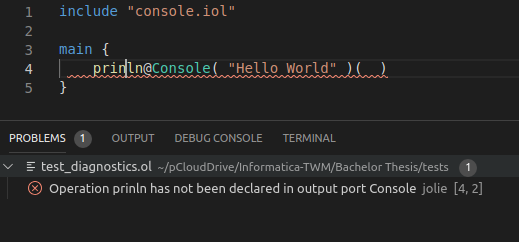
\includegraphics[width=\textwidth]{tests/screenshots/diagnostics_final.png}
	\caption{FR 1 diagnostics}
	\label{FR1Val}
\end{figure}

\subsection{FR 2 and FR 3}
FR 2 and 3 are fully met. See Figure \ref{FR2Val} and Figure \ref{FR2Val_res} for FR2, Figure \ref{FR3Val} and Figure \ref{FR3Val_res} for FR3.
\begin{figure}[t]
	\centering
	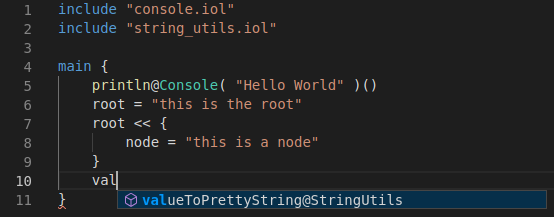
\includegraphics[width=\textwidth]{tests/screenshots/completion_operation_cropped.png}
	\caption{FR 2 completion list}
	\label{FR2Val}	
\end{figure}
\begin{figure}[t]
	\centering
		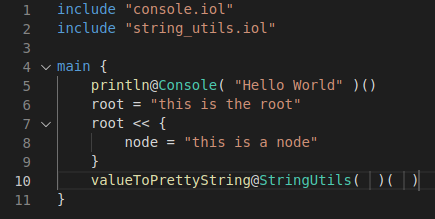
\includegraphics[width=\textwidth]{tests/screenshots/compl_operation_result_cropped.png}
	\caption{FR 2 snippet}
	\label{FR2Val_res}
\end{figure}
\begin{figure}[t]
	\centering
	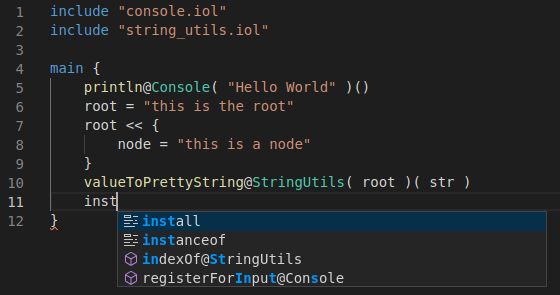
\includegraphics[width=\textwidth]{tests/screenshots/completion_keywords_cropped.png}
	\caption{FR 3 completion list}
	\label{FR3Val}
\end{figure}
\begin{figure}[t]
	\centering
	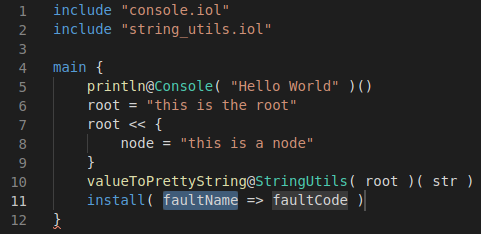
\includegraphics[width=\textwidth]{tests/screenshots/completion_keywords_result_cropped.png}
	\caption{FR 3 snippet}
	\label{FR3Val_res}
\end{figure}
\subsection{FR 4}
This is managed by the Utils service. In order to verify the requirement, URIs of the actual documents saved in the server memory were printed in the console every time a \verb|didOpen| or \verb|didClose| message were received. Figure \ref{FR4Val_1} shows that after opening the third document, the Language Server prints the URIs of the documents in memory and when the file \emph{utils.iol} is closed, it prints the URIs of the remaining two, as shown in \hyperref[FR4Val_2]{figure 6.7}. Utils uses the \emph{Inspector} service for generating a data structure containing all the information regarding the \textbf{deployment}, and no information regarding the \textbf{behavior}.
\begin{figure}[t]
	\centering
	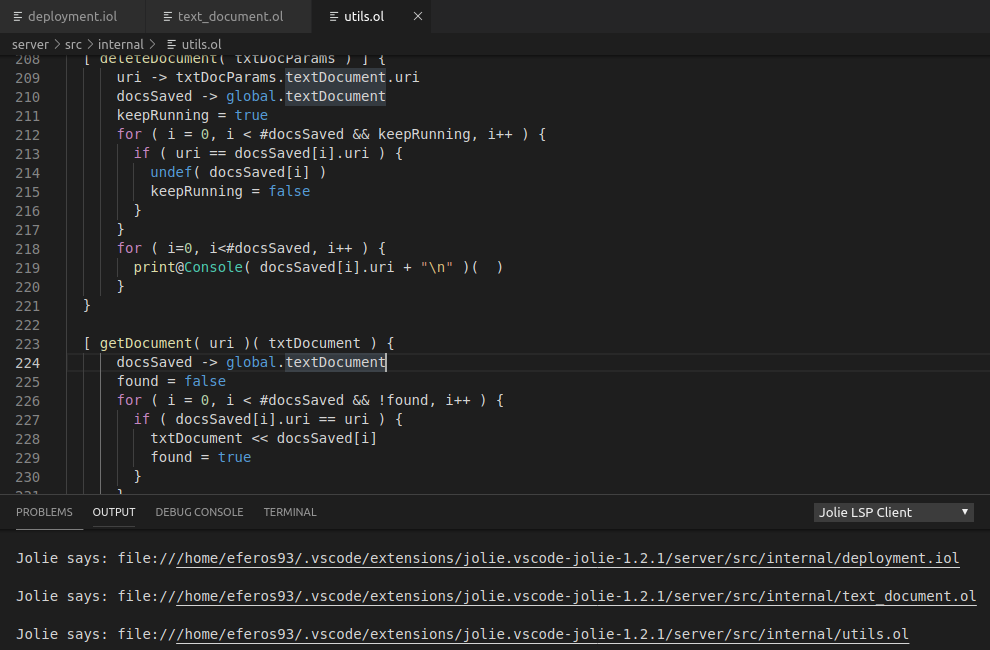
\includegraphics[width=\textwidth]{tests/screenshots/synch_1.png}
	\caption{synchronization didOpen}
	\label{FR4Val_1}
\end{figure}
\begin{figure}[t]
	\centering
	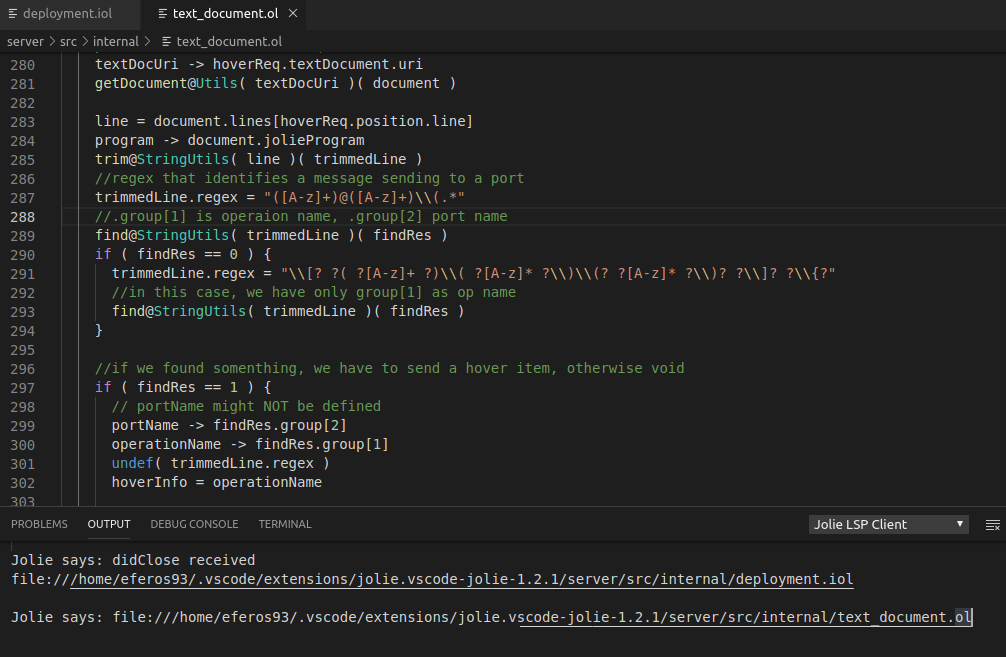
\includegraphics[width=\textwidth]{tests/screenshots/synch_2.png}
	\caption{synchronization didClose}
	\label{FR4Val_2}
\end{figure}

\subsection{FR 5}
FR 5 is met, as shown by \hyperref[FR5Val]{figure 6.8}.
\begin{figure}[t]
	\centering
	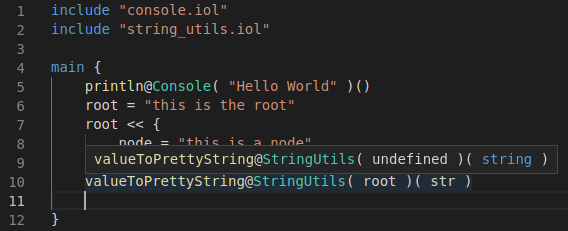
\includegraphics[width=\textwidth]{tests/screenshots/hover_cropped.png}
	\caption{FR 5 hover information}
	\label{FR5Val}
\end{figure}
\subsection{Unmet Functional requirements: FR 6, 7 and 8}
Functional requirements 6, 7 and 8 are unmet. This is due to the fact that at the moment it is not possible to provide a hierarchy or symbols to the client and there was not enough time to develop such functionality. The \verb|Inspector| service, provides a syntax check and a full description of the deployment part, but not of the behavior, namely it is not possible to identify the symbols and their location.
\section{Non-Functional requirements}
The non-functional requirements defined in \hyperref[sec:NFR]{Chapter 3} are all met, except for NFR 4 (partial) and 5 (unmet), as Table \ref{NFRVal} shows.
\begin{table}[t]
	\caption{Non-Functional Requirements}
	\label{NFRVal}
	\begin{tabularx}{\textwidth}{c|c|X}
		\hline
		& \textbf{Non-functional r. No.} & \textbf{Description}\\
		\hline\hline
		\greenc & NFR 1 & The server must support the LSP's JSON-RPC protocol.\\\hline
		\greenc & NFR 2 & The server must be designed to be modular.\\\hline
		\greenc & NFR 3 & The server must be able to respond to a client request as soon as possible.\\\hline
		\orangec & NFR 4 & The server must work both when deployed in a different machine and when deployed in a local machine, with respect of the client location. As a consequence, it has to support the socket channel of communication.\\\hline
		\redx & NFR 5 & The server must be able to handle more clients sending multiple requests concurrently.\\\hline
	\end{tabularx}
\end{table}

The actual implementation of the server corresponds to the local architecture presented in \hyperref[sec:arch]{Chapter 4}, there was not enough time to develop and test the distributed one. Despite this, it should not be difficult to develop it, as it would just require to deploy the local server implementation in a remote machine and create a \emph{Proxy Service} located in the clients machine, which stands in between of the development tool and the server. NFR 5 is a direct consequence of the previous requirements. However, setting the execution modality both of the proxy and of the server to \emph{concurrent}.
\chapter{Conclusions}
In this thesis we have provided a LS for Jolie, an innovative programming language for developing distributed system based on microservice architectures. The LS we have developed adapts the Language Server Protocol, a JSON-RPC-based protocol that standardizes the communication between an IDE and a Language Server.
\section{Project review}
The project consisted in:
\begin{enumerate}
	\item extracting the requirements for the Jolie Language Server, where functional ones where dictated by the Language Server Protocol Specifications while the non-functional ones were established together with the internship supervisor, in order to have a software that can be \textbf{easily extended} with new \textbf{capabilities};
	\item modeling the software architecture that reflects the requirements defined, especially the non-functional ones. The architecture was therefore based on microservices;
	\item due to the nature of the architecture, Jolie was the preferred programming language to be used for the implementation. This required some improvements in the Jolie JSON-RPC protocol in order to make it compatible with the LSP counterpart. Those improvements included:
	\begin{enumerate}
		\item creating two new classes, \verb|LSPMessage| and \verb|LSPParser|, which respectively represent a full LSP message and its parser;
		\item modifying \verb|JsonRpcProtocol| class in order to handle the LSP messages by using the classes mentioned above, including some improvements when converting a Jolie value to a JSON string and vice-versa;
	\end{enumerate}	 
	\item the language features implemented were the \textbf{completion} for keywords and operations, \textbf{hover} functionality for operations and  \textbf{diagnostics}, providing linting for errors in the code;
	\item the program was tested on itself and also by writing simple ones.
\end{enumerate} 


\section{Unmet requirements}
Capabilities like the \textbf{go-to definition} and \textbf{find references} have not been implemented due to the lack of a tool for obtaining an Abstract Syntax Tree of the behavior. As a consequence, completion feature is supported only for \textbf{output ports} and \textbf{keywords}, while it is not possible to auto-complete variables. Regarding the architecture, only the local one presented in \hyperref[sec:arch]{Chapter 4} was implemented.

\section{Future Work}
Future work includes extending the Jolie library, refactoring the actual Language Server code and implementing the \hyperref[distrArch]{distributed architecture}.

The first consists in integrating the Inspector service in order to be able to provide, together with information regarding the deployment, a data structure representing the \emph{Abstract Syntax Tree} of the program, from which, by extending the completion operation, the Language Server will be able to provide also a list of possible completion items for variables. This can be done by interfacing the Inspector with Jolie's front end i.e. the Jolie parser. As a consequence, the LS can be extended in order to create a hierarchy of symbols to be sent to the development tool, granting the possibility to implement features like \textbf{go-to definition} and \textbf{find references}.

The second consists of refactoring the actual searching algorithm, which is a simple \textit{linear search}, to a more sophisticated one, like the \textit{Approximate String Matching}, also referred as Fuzzy search. The general goal is to perform string matching of a pattern in a text where one or both of them have suffered some kind of (undesirable) corruption \cite{Navarro99aguided}. Another improvement can consists in generating a sorted list of operations from the Inspector response and then implement a Binary Search algorithm when generating the completion list to be sent to the client. However, this sorting would be applied every time an inspection is executed, namely every time a \verb|didOpen| or \verb|didChange| message is received. Furthermore, the \verb|didChange| message is sent every time a single char is typed. Therefore another improvement may consist in implementing a mechanism that lets the LS update its state just for some of the \verb|didChange| messages received. More in depth, when the LS starts, a \emph{change bit} is set to 1 and a timer is set. When we receive the first \verb|didChange| message, we start the timer, update the state and set the change bit to 0. When the timer elapses, we reset it and we set the change bit back to 1. If we receive another \verb|didChange| before the timer is elapsed, the message is discarded, otherwise the behavior is same as the one described above. Following the pseudo code:
\begin{algorithm}[H]
\caption{ChangeBit}
\begin{algorithmic}
\If {$changeBit == 1$}
	\State $startTimer()$
	\State $updateState()$
	\State $changeBit \gets 0$
\Else
	\State $discardMessage()$
\EndIf
\end{algorithmic}
\end{algorithm}
This will avoid useless computations by the LS and it can be implemented in both architectures: in the distributed one in the Proxy Service, while in the local in the Main Service.

Last but not least, the implementation of the distributed architecture. This requires the implementation of the \emph{Proxy Service} and a mechanism to handle sessions. In Jolie they can be implemented with \emph{Correlation Sets}. For more details about this, see \cite{Jol, JolieDoc}.
\appendix

%\part{Appendici}

%\chapter{Altro capitolo}

%% Parte conclusiva del documento; tipicamente per riassunto, bibliografia e/o indice analitico.
\backmatter

%% Riassunto (opzionale)
%\summary

%% Bibliografia (opzionale)
\bibliographystyle{plain_\languagename}%% Carica l'omonimo file .bst, dove \languagename � la lingua attiva.
%% Nel caso in cui si usi un file .bib (consigliato)
\bibliography{thud}
%% Nel caso di bibliografia manuale, usare l'environment thebibliography.

%% Per l'indice analitico, usare il pacchetto makeidx (o analogo).

\end{document}

--- Istruzioni per l'aggiunta di nuove lingue ---
Per ogni nuova lingua utilizzata aggiungere nel preambolo il seguente spezzone:
    \addto\captionsitalian{%
        \def\abstractname{Sommario}%
        \def\acknowledgementsname{Ringraziamenti}%
        \def\authorcontactsname{Contatti dell'autore}%
        \def\candidatename{Candidato}%
        \def\chairname{Direttore}%
        \def\conclusionsname{Conclusioni}%
        \def\cosupervisorname{Co-relatore}%
        \def\cosupervisorsname{Co-relatori}%
        \def\cyclename{Ciclo}%
        \def\datename{Anno accademico}%
        \def\indexname{Indice analitico}%
        \def\institutecontactsname{Contatti dell'Istituto}%
        \def\introductionname{Introduzione}%
        \def\prefacename{Prefazione}%
        \def\reviewername{Controrelatore}%
        \def\reviewersname{Controrelatori}%
        %% Anno accademico
        \def\shortdatename{A.A.}%
        \def\summaryname{Riassunto}%
        \def\supervisorname{Relatore}%
        \def\supervisorsname{Relatori}%
        \def\thesisname{Tesi di \expandafter\ifcase\csname thud@target\endcsname Laurea\or Laurea Magistrale\or Dottorato\fi}%
        \def\tutorname{Tutor aziendale%
        \def\tutorsname{Tutor aziendali}%
    }
sostituendo a "italian" (nella 1a riga) il nome della lingua e traducendo le varie voci.
